\title{調達資金の時間変化測定に基づくクラウドファンディングの成功要因分析}
\author{プロジェクトマネジメントコース\\
ソフトウェア開発管理グループ\\
矢吹研究室\\
1342066\\
島田樹}
\date{}
\begin{document}
\maketitle

%本テンプレートの余白は,卒論マニュアルで指示されたものとは違っているが,1ページあたりの文字数は40文字x40行と,卒論マニュアル通りになっている。文字間隔や行間隔を調整して,余白をマニュアル通りにすることもできるが,それでは文章が読みにくくなるため,このような対応をしている。

%\noindent
□□□□□□□□□■□□□□□□□□□■□□□□□□□□□■□□□□□□□□□■
□□□□□□□□□■□□□□□□□□□■□□□□□□□□□■□□□□□□□□□■
□□□□□□□□□■□□□□□□□□□■□□□□□□□□□■□□□□□□□□□■
□□□□□□□□□■□□□□□□□□□■□□□□□□□□□■□□□□□□□□□■
□□□□□□□□□■□□□□□□□□□■□□□□□□□□□■□□□□□□□□□■
□□□□□□□□□■□□□□□□□□□■□□□□□□□□□■□□□□□□□□□■
□□□□□□□□□■□□□□□□□□□■□□□□□□□□□■□□□□□□□□□■
□□□□□□□□□■□□□□□□□□□■□□□□□□□□□■□□□□□□□□□■
□□□□□□□□□■□□□□□□□□□■□□□□□□□□□■□□□□□□□□□■
□□□□□□□□□■□□□□□□□□□■□□□□□□□□□■□□□□□□□□□■
□□□□□□□□□■□□□□□□□□□■□□□□□□□□□■□□□□□□□□□■
□□□□□□□□□■□□□□□□□□□■□□□□□□□□□■□□□□□□□□□■
□□□□□□□□□■□□□□□□□□□■□□□□□□□□□■□□□□□□□□□■
□□□□□□□□□■□□□□□□□□□■□□□□□□□□□■□□□□□□□□□■
□□□□□□□□□■□□□□□□□□□■□□□□□□□□□■□□□□□□□□□■
□□□□□□□□□■□□□□□□□□□■□□□□□□□□□■□□□□□□□□□■
□□□□□□□□□■□□□□□□□□□■□□□□□□□□□■□□□□□□□□□■
□□□□□□□□□■□□□□□□□□□■□□□□□□□□□■□□□□□□□□□■
□□□□□□□□□■□□□□□□□□□■□□□□□□□□□■□□□□□□□□□■
□□□□□□□□□■□□□□□□□□□■□□□□□□□□□■□□□□□□□□□■
□□□□□□□□□■□□□□□□□□□■□□□□□□□□□■□□□□□□□□□■
□□□□□□□□□■□□□□□□□□□■□□□□□□□□□■□□□□□□□□□■
□□□□□□□□□■□□□□□□□□□■□□□□□□□□□■□□□□□□□□□■
□□□□□□□□□■□□□□□□□□□■□□□□□□□□□■□□□□□□□□□■
□□□□□□□□□■□□□□□□□□□■□□□□□□□□□■□□□□□□□□□■
□□□□□□□□□■□□□□□□□□□■□□□□□□□□□■□□□□□□□□□■
□□□□□□□□□■□□□□□□□□□■□□□□□□□□□■□□□□□□□□□■
□□□□□□□□□■□□□□□□□□□■□□□□□□□□□■□□□□□□□□□■
□□□□□□□□□■□□□□□□□□□■□□□□□□□□□■□□□□□□□□□■
□□□□□□□□□■□□□□□□□□□■□□□□□□□□□■□□□□□□□□□■
□□□□□□□□□■□□□□□□□□□■□□□□□□□□□■□□□□□□□□□■
□□□□□□□□□■□□□□□□□□□■□□□□□□□□□■□□□□□□□□□■
□□□□□□□□□■□□□□□□□□□■□□□□□□□□□■□□□□□□□□□■
□□□□□□□□□■□□□□□□□□□■□□□□□□□□□■□□□□□□□□□■
□□□□□□□□□■□□□□□□□□□■□□□□□□□□□■□□□□□□□□□■
□□□□□□□□□■□□□□□□□□□■□□□□□□□□□■□□□□□□□□□■
□□□□□□□□□■□□□□□□□□□■□□□□□□□□□■□□□□□□□□□■
□□□□□□□□□■□□□□□□□□□■□□□□□□□□□■□□□□□□□□□■
□□□□□□□□□■□□□□□□□□□■□□□□□□□□□■□□□□□□□□□■
■■■■■■■■■■■■■■■■■■■■■■■■■■■■■■■■■■■■■■■■
□□□□□□□□□■□□□□□□□□□■□□□□□□□□□■□□□□□□□□□■%文字数チェック用

\tableofcontents%目次


\chapter{序論}
当研究は,調達資金の時間変化測定に基づくクラウドファンディングの成功要因分析を行う.
クラウドファンディングはプロジェクトの資金をインターネットを通じて,不特定多数から募る手法である.クラウドファンディングを活用することで,製品やサービスの開発に必要な資金を集めることができるだけでなく、より多くの人へ向けて自身の背品やサービスを認知してもらうことができる.
当研究では,プロジェクト実行者が資金を集めるために行っている行動を調査する.調達資金を可視化し,実行者がした行動を分析することによって成功要因を導き出す.

%-------------------------------------------------------------------------------------------------------------------------------------------
\chapter{背景}
クラウドファンディングは,SNS の発達に伴いプロジェクトの数も増加し,市場も年々増加している\cite{visualizing}.幅広い分野と規模での応募が可能で,ベンチャー企業のプロジェクトや学生の研究費用の獲得などが多かったが,大手企業も支援者数から売れることを確実視されたプロダクトを販売者できるとして,マーケティングの一環として活用されるようになってきた.



%-------------------------------------------------------------------------------------------------------------------------------------------
\chapter{クラウドファンディングについて}
\section{クラウドファンディングとは}
クラウドファンディングとは\cite{wiki},群衆と資金調達を組み合わせた造語で,クリエイターや起業家が製品・サービスの開発,もしくはアイデアの実現などの「ある目的」のために,インターネットを通じて不特定多数の人から資金の出資や協力を募ることをいう.

例として何か製品を作る場合に,何故その製品を作るのか,どのような製品を作るのか,どのように作っていくのか,資金はいくら必要なのか,といった情報をプロジェクトとしてクラウドファンディングサービス上に掲載する.出資をしてくれた人に対して何か見返り(リターン)がある場合はその旨も記載する.一定期間の間に,プロジェクトに共感した複数人の支援者が少額づつ資金を出資・支援し,目的の資金が集まった時点でプロジェクトが成立し,プロジェクトの起案者は,集まった資金を元手にプロジェクトを実行する.その際,プロジェクト起案者は,サービス運営者に,集まった金額の10〜20%を手数料として支払う.

\begin{figure}[htb]
\centering
\includegraphics[width=13cm]{cloud.pdf}
\caption{クラウドファンディングの仕組み}\label{サンプル図}
\end{figure}

\section{クラウドファンディングの種類}
クラウドファンディングは,一般的には支援者に対するリターンによって3つに分類される\cite{shurui}.
\begin{description}
 \item 金銭的リターンのない 「寄付型」
 \item 金銭的リターンのある 「投資型」
 \item 権利や物品を購入することで支援する 「金融型」
\end{description}

\subsection{寄付型クラウドファンディング}
寄付型クラウドファンディングは,プロジェクトに対して出資を行うが,あくまでも寄付であるためリターンは発生しない.
被災地支援や発展途上国の支援などの社会的意義の大きいプロジェクトとの相性がいい.
通常の寄付であれば,寄付金の使い道が分かりづらいことが多いが,クラウドファンディングを利用することで,寄付後のプロジェクトの状況が透明化される.

\subsection{購入型クラウドファンディング}
購入型クラウドファンディングは,支援者がプロジェクトへの出資することで支援金額に応じた金銭以外の商品やサービスが手に入る.
クラウドファンディングは,プロジェクト成功後に商品の作成が多いので,先行販売という形に近い.
日本国内で一番採用されているタイプである.

\subsection{金融型クラウドファンディング}
金融型クラウドファンディングは,支援者が特定の企業などに出資を行い,リターンとして金銭(配当や利益の一部)または株式が発行される.
今までは比較的大きい投資などが必要で,個人ではハードルが高かった投資を小口から出資できるようになったことで誰でも投資活動ができるようになるのが特徴である.
誰でも未公開企業に対して株式という形で投資ができるので,非常に注目が集まっているが,日本においては2014年に金融商品取引法が改正されるまでは寄付型と購入型に限られていた.


\section{クラウドファンディングの歴史}
クラウドファンディングのような仕組みは,17世紀初頭から始まっている.書籍編集者のジョン・テイラー氏が,書籍の印刷代を寄付によって集めた事例がクラウドファンディングの原型と言われている\cite{rekishi}.そしてアメリカで2006年に企業家のマイケル・サリバンが初めて「クラウドファンディング」という言葉を用いた.大手クラウドファンディングサービスは,2008年に「IndieGoGo」,翌年2009年に「Kickstarter」がリリースされている.
日本では2011年4月にリリースされた「READYFOR」が最初のクラウドファンディングサービスである.




%-------------------------------------------------------------------------------------------------------------------------------------------
\chapter{目的}
先行研究\cite{miura}ではプロジェクトの内容以外の要因を調査し,目標金額等の設定段階で成功率を上げることを目的としていた.本研究では調達資金の時間変化を可視化し,動画の投稿やSNSでの告知などの多くの資金を集める直前に行っているプロジェクト実行者の行動を分析する.その結果から,プロジェクト実行者が資金を集める際の参考となる指標を作ることを目的とする.



%-------------------------------------------------------------------------------------------------------------------------------------------
\chapter{手法}
初めにクラウドファンディングサイトを,毎日定時に監視し,データ収集を行う.収集したデータから成功しているプロジェクトの資金調達を可視化し,資金が集まり始めるときにしている行動を調査する.調査項目は,サイト内のレポートを活用しているか,動画を投稿しているか,Twitterでツイートをしているか,Facebookで投稿しているか,の4項目である.この4項目に調達金額を目標金額で割った目標達成率を足した5項目から決定木を作成し,調達資金に必要な行動を考察する.

\newpage

\section{Chocolateyについて}
\subsection{Chocolateyとは}
ChocolateyはWindowsのためのパッケージ管理ツールである.Chocolateyを使うことによってWindows上で動作するソフトウェアをコマンドラインからインストール,アンインストール,アップデート,検索を行うことができる.

\subsection{Chocolateyのインストール}
Windowsのコマンドプロンプトを管理者として実行する.

\begin{figure}[h]
\centering
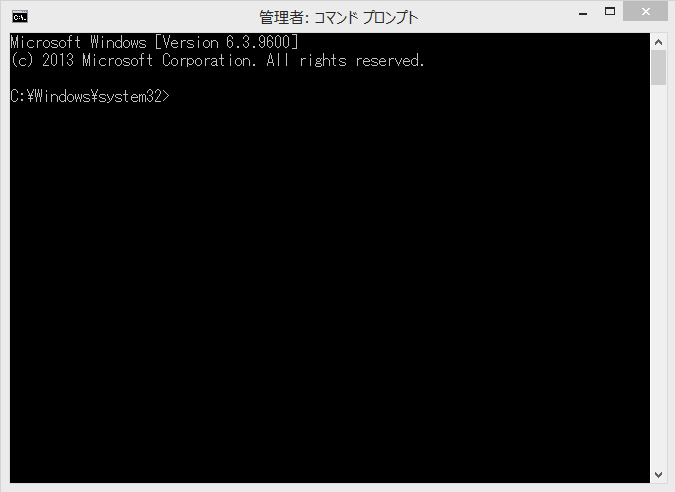
\includegraphics[width=12cm]{choco1.PNG}
\caption{管理者で起動したコマンドプロンプト}\label{サンプル図}
\end{figure}

\newpage


\begin{figure}[h]
\centering
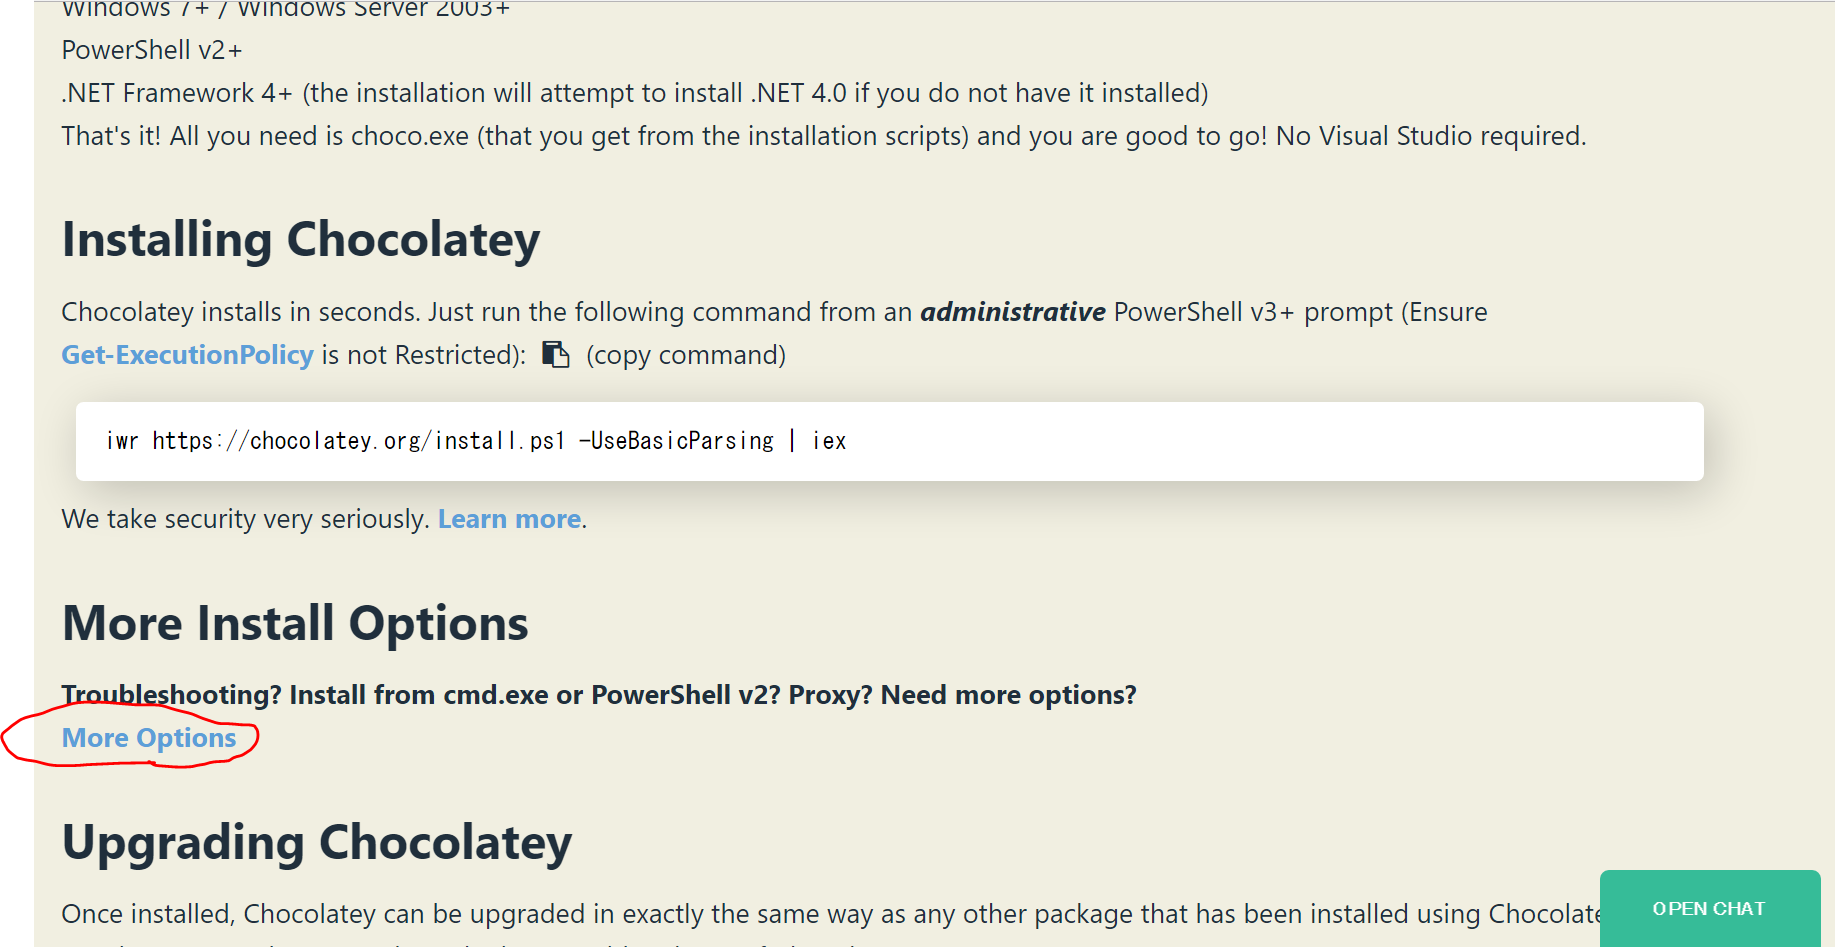
\includegraphics[width=12cm]{choco2.PNG}
\caption{ダウンロードサイト1}\label{サンプル図}
\end{figure}

https://chocolatey.org/ を入力してchocolateyのサイトを表示し,Install Chocolatey Nowをクリックする.

\newpage

\begin{figure}[h]
\centering
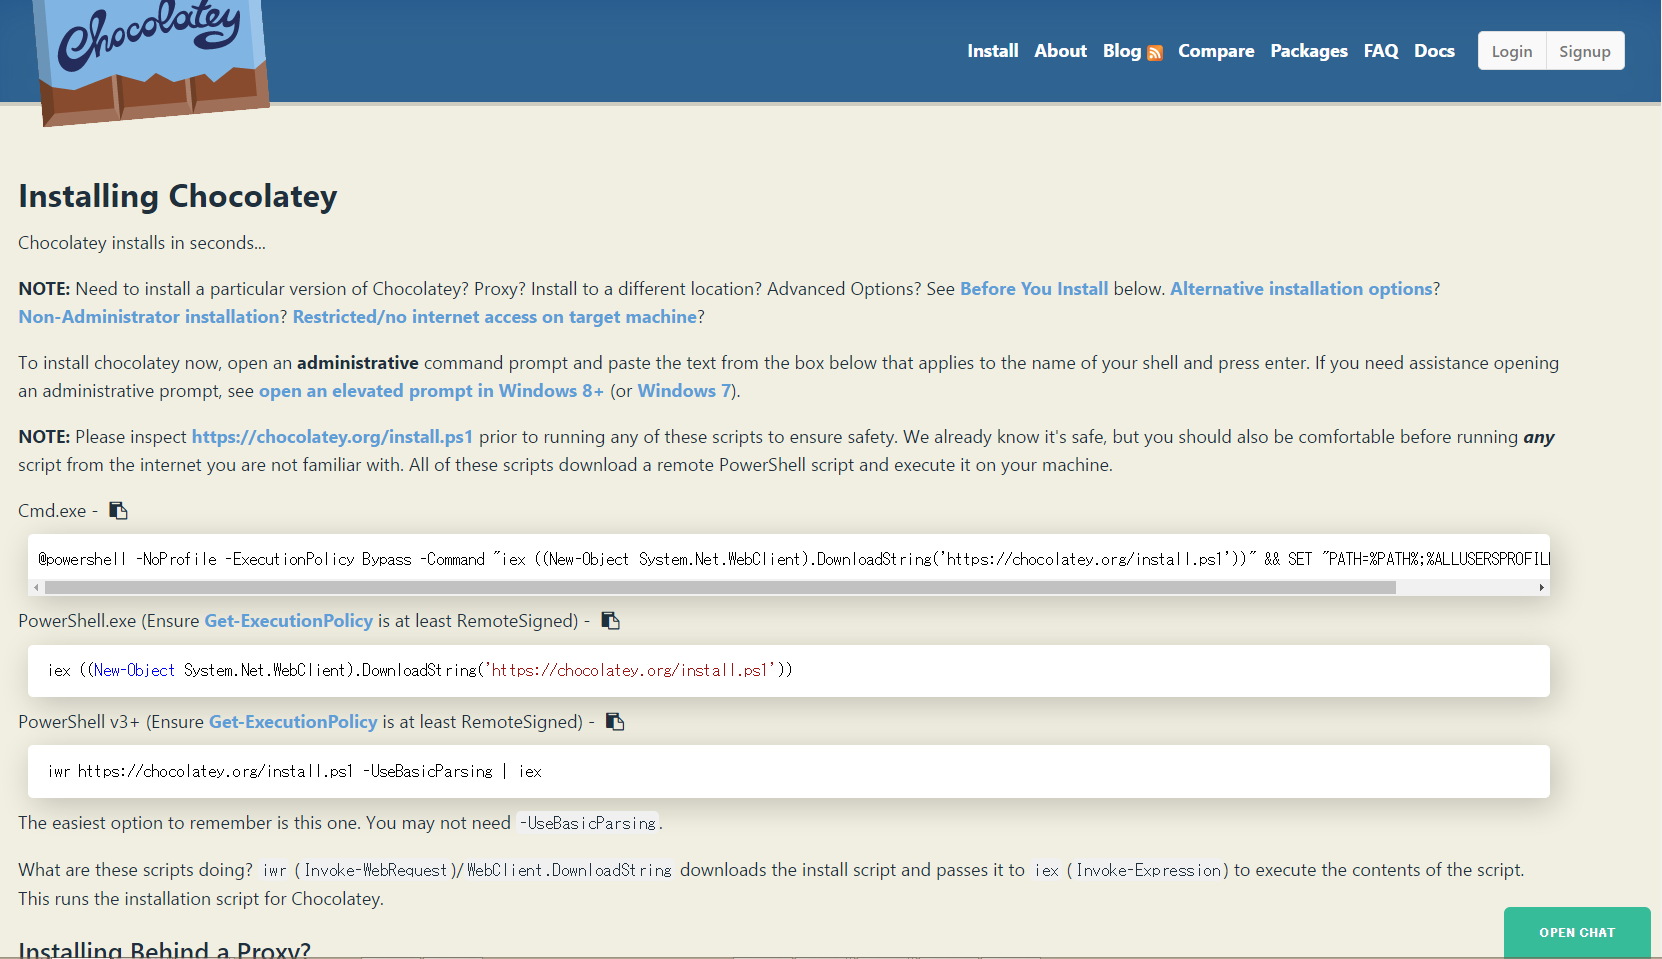
\includegraphics[width=12cm]{choco3.PNG}
\caption{ダウンロードサイト2}\label{サンプル図}
\end{figure}





\newpage

\begin{figure}[h]
\centering
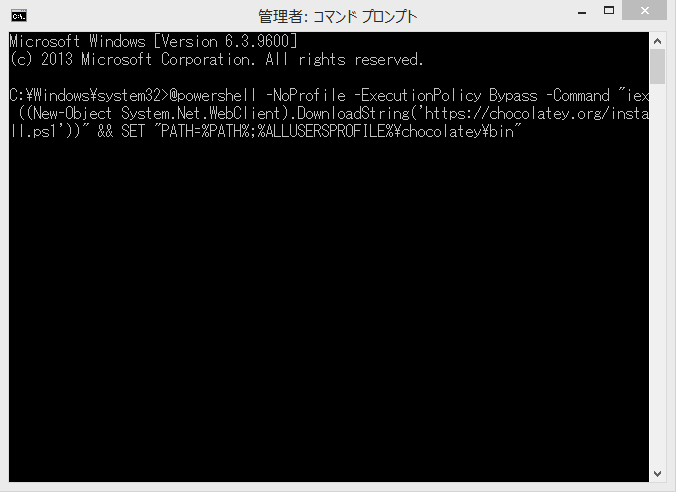
\includegraphics[width=12cm]{choco4.PNG}
\caption{コマンドプロンプト}\label{サンプル図}
\end{figure}

Cmd.exeに書かれているコマンドをコピーし,起動したコマンドプロンプトで実行する.

\newpage

\section{VirtualBoxについて}
\subsection{VirtualBoxとは}
VirtualBoxは,使用しているPC上に仮想的なPCを作成し,別のOSをインストール・実行できるフリーの仮想化ソフトである.

VirtualBoxはコンピュータ上で直接動作している通常のOSにとってはアプリケーションソフトの一つであり,他のソフトと同じように起動することができる.起動すると仮想的なコンピュータが構築され,元のOSとは独立に別のOSを起動することができる.VirtualBoxが実行されているOSをホストOS,VirtualBox上で実行されているOSをゲストOSという.

\begin{figure}[h]
\centering
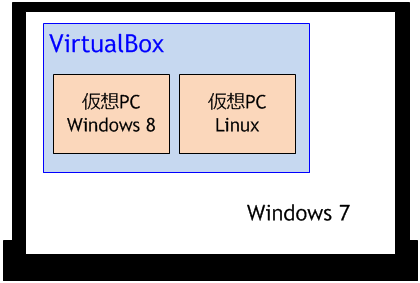
\includegraphics[width=10cm]{virtualbox1.png}
\caption{仮想マシンのイメージ}\label{サンプル図}
\end{figure}

元は独立系のソフトウェア企業が開発・販売していた製品だったが,開発元がSun Microsystems社に買収され,その後同社がOracle社に買収されたため,Oracle社が開発元となり,正式名称も「Oracle VM VirtualBox」となった.また,VirtualBox本体はGPLに基いてオープンソースソフトウェアとして公開され,誰でも自由に入手・利用・改変・再配布などが行える.同社ではVirtualBoxに機能を追加するソフトウェアを製品として開発・販売している.

\newpage

\section{VirtualBoxのインストール}
本研究ではChocolateyを使用してインストールする.

コマンドプロンプトを管理者で起動する.


\begin{figure}[h]
\centering
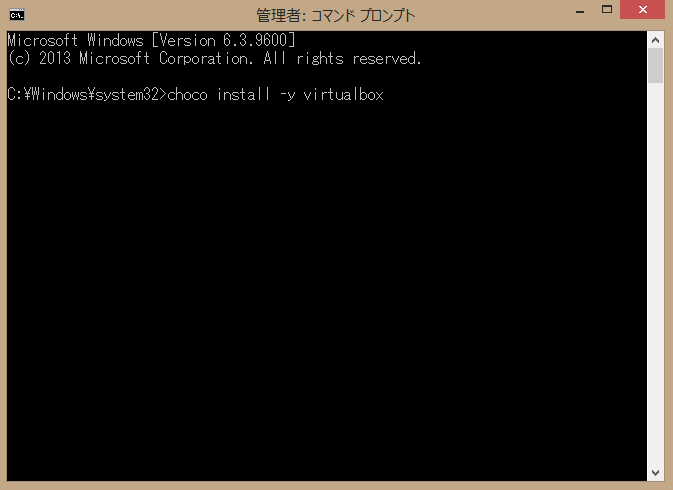
\includegraphics[width=12cm]{virtualbox2.PNG}
\caption{VirtualBoxのインストール1}\label{サンプル図}
\end{figure}

\newpage


choco install -y virtualbox と入力し実行する

\begin{figure}[h]
\centering
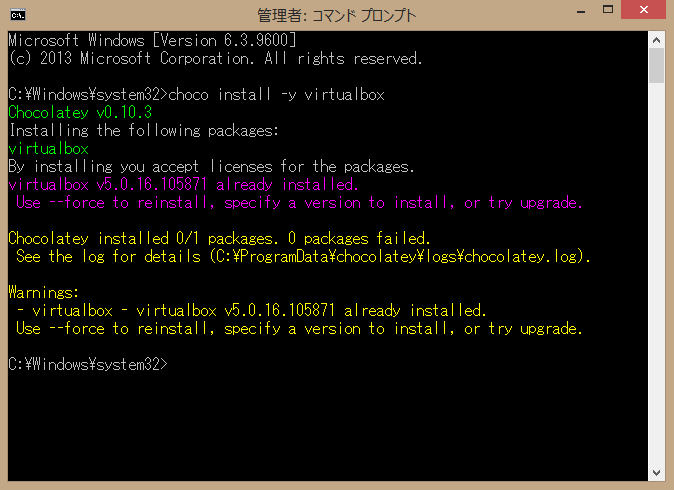
\includegraphics[width=12cm]{virtualbox3.PNG}
\caption{VirtualBoxのインストール2}\label{サンプル図}
\end{figure}

このようになればインストール完了

\newpage

\section{Vagrantについて}
\subsection{Vagrantとは}
Vagrantとは,仮想環境を作成するにあたって,簡単に構築・管理し配布することができるツールである.VirtualBoxとVagrantの2つがあることで,開発環境を仮想マシン上に自動作成することができる.


\subsection{Vagrantのインストール}
本研究ではChocolateyを使用してインストールする.
コマンドプロンプトを管理者で起動する.

\begin{figure}[h]
\centering
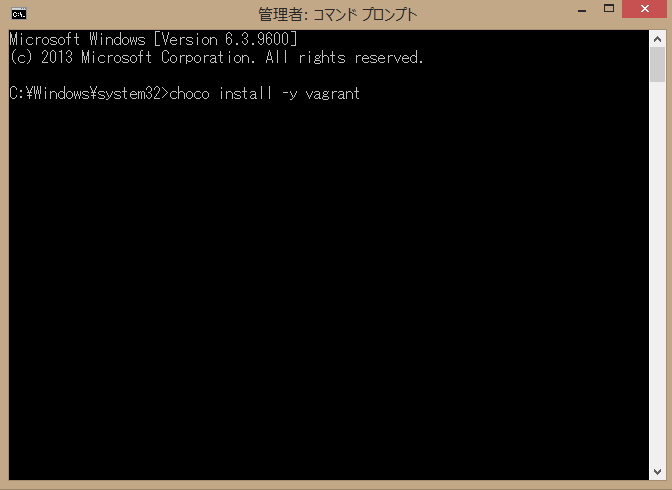
\includegraphics[width=12cm]{vagrant1.PNG}
\caption{Vagrantのインストール1}\label{サンプル図}
\end{figure}

choco install -y vagrant と入力し実行する

\newpage

\begin{figure}[h]
\centering
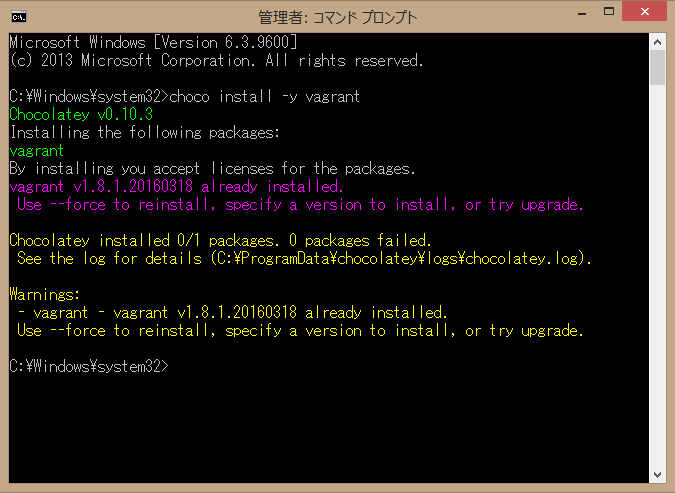
\includegraphics[width=12cm]{vagrant2.PNG}
\caption{Vagrantのインストール}\label{サンプル図}
\end{figure}

このようになればインストール完了


\section{R言語について}
\subsection{R言語とは}
R言語とは、統計解析やその結果をグラフィカルに表示するためのシステム「R」用の言語のことである。R言語は、AT\&Tベル研究所の研究者によって設計された統計処理言語であるS言語を元に設計されている。同じくAT\&Tベル研究所のが開発した「S言語」の実装系は商用版が知られているが、R言語はGNUプロジェクトによってオープンソースで提供されており、無償で利用できる。R言語は見かけはC言語に似ているが、簡単なコマンドによりいろいろな機能が実現できる。標準では用意されていない機能も比較的容易に拡張できるメリットがある。

\newpage

\subsection{Rのインストール}
RはWindows、Mac、Unixのすべてに対応している.本研究ではWindows版を使用する.
RjpWiki\cite{Rjp}にアクセスしRをインストールしていく.

\begin{figure}[H]
\centering
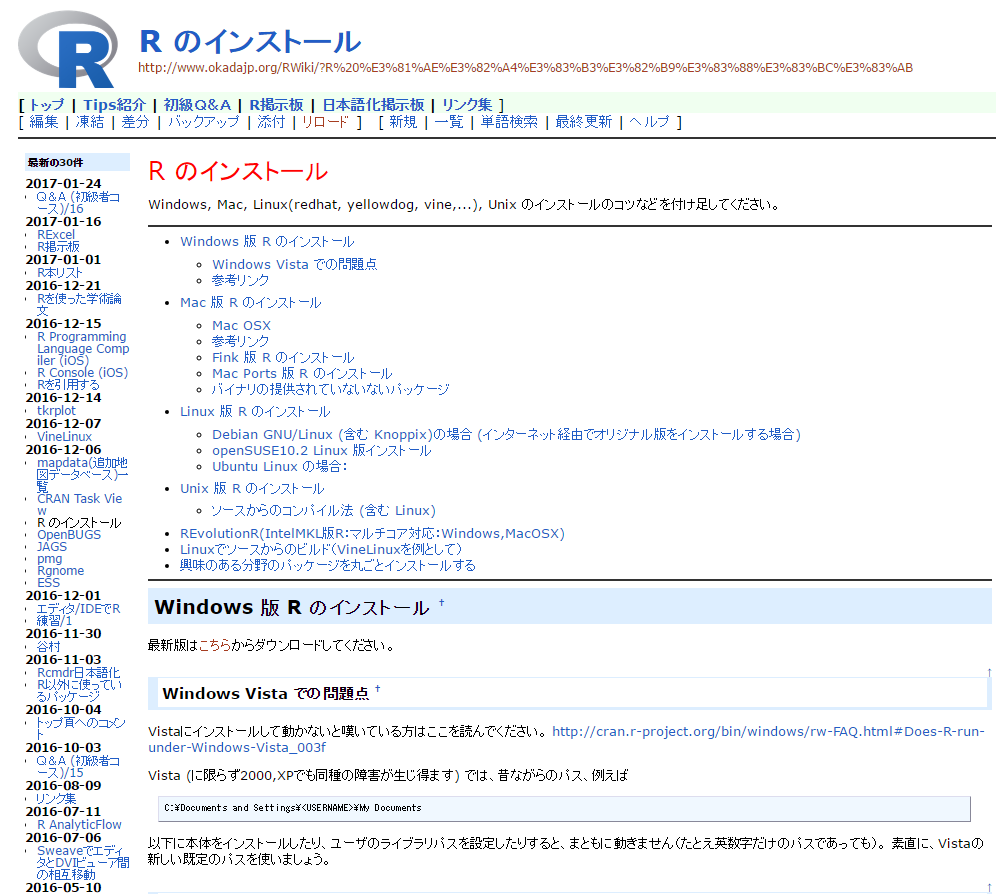
\includegraphics[width=12cm]{R1.PNG}
\caption{Rインストール手順1}\label{サンプル図}
\end{figure}

Windows版Rの最新版リンクをクリックする.

\newpage

\begin{figure}[H]
\centering
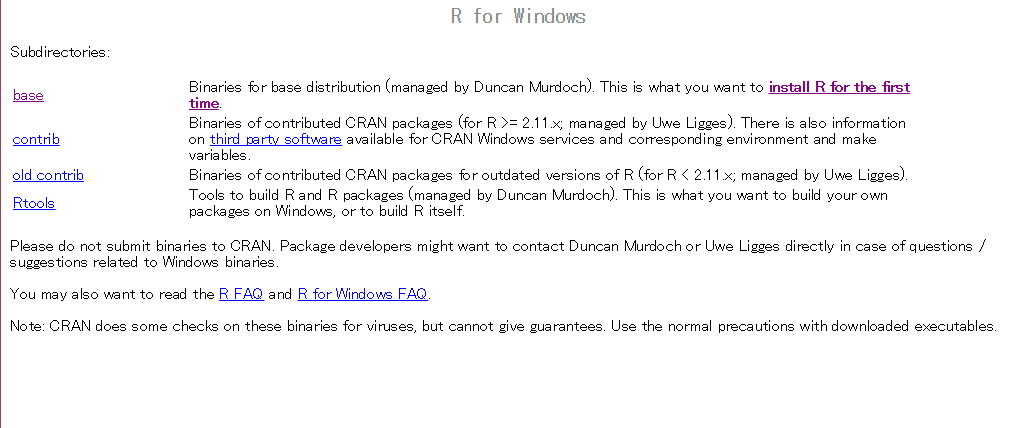
\includegraphics[width=12cm]{R2.PNG}
\caption{Rインストール手順2}\label{サンプル図}
\end{figure}

install R for the first time.をクリックする.

\begin{figure}[H]
\centering
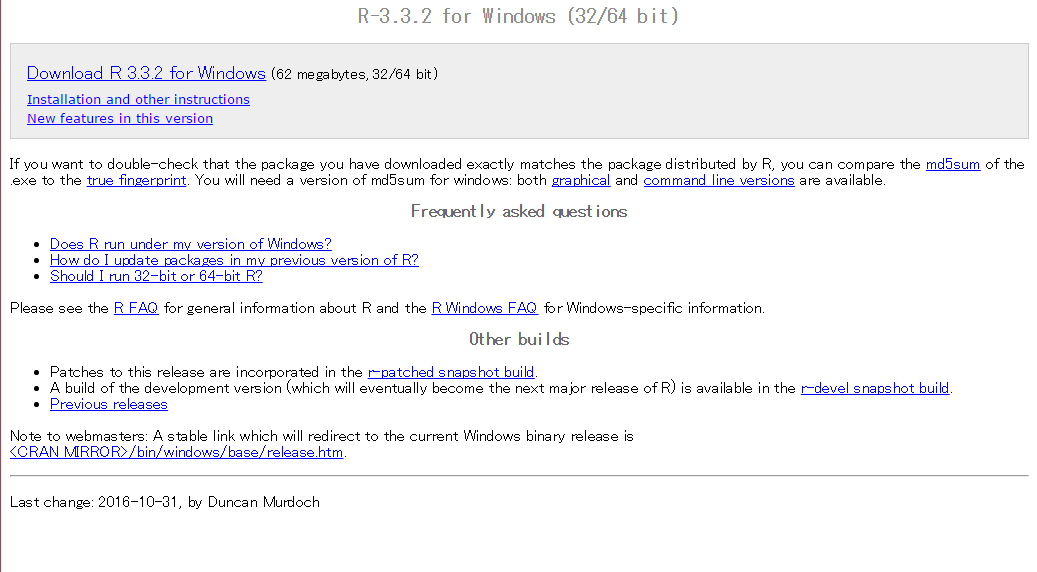
\includegraphics[width=12cm]{R3.PNG}
\caption{Rインストール手順3}\label{サンプル図}
\end{figure}

Download R 3.3.2 for Windowsをクリックするとダウンロードが始まる.

\newpage

\begin{figure}[H]
\centering
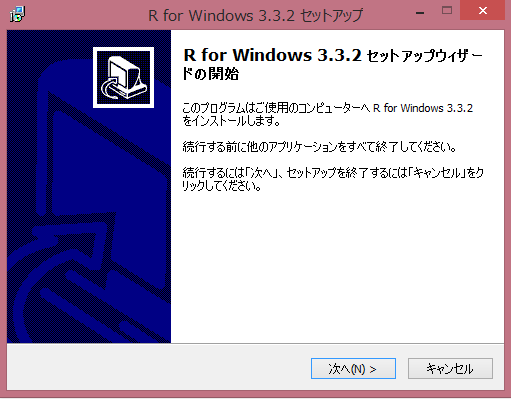
\includegraphics[width=12cm]{R4.PNG}
\caption{Rインストール手順4}\label{サンプル図}
\end{figure}

ダウンロードしたexeを起動し,セットアップをすることでインストール完了する.
%-----------------------------------------------------------------------------------------------------------------------------

\newpage
\section{クローラーについて}
\subsection{クローラーとは}
クローラー(Crawler)とは、ウェブ上の文書や画像などを周期的に取得し、自動的にデータベース化するプログラムである。「ボット(Bot)」、「スパイダー」、「ロボット」などとも呼ばれる。主に検索エンジンのデータベース、インデックス作成に用いられているほか、統計調査などの目的にも利用される。近年では電子メールアドレス収集業者などもクローラを利用して、スパムの送信効率を上げている。 
一般にクローラは、既知のHTML文書の新しいコピーを要求し、文書中に含まれるリンクをたどり別の文書を収集するという動作を繰り返す。新しい文書を見つけた場合はデータベースに登録する。また、既知のファイルが存在しないことを検出した場合はデータベースから削除する\cite{crawler}。 クローラーとして最も有名なのは,Google などの検索エンジンがあげられる.
本研究ではフリーソフトであるwgetを利用しクローラーを作成する.

\subsection{wgetとは}
HTTP/HTTPSとFTPで利用できるファイル取得用コマンド「wget」は、その多機能さと移植性の高さにより、Linuxを始めとする多くのUNIX系OSで利用されている。また、Windows OS環境向けには「Wget for Windows」が配布されている。
wgetは、ソースコードやバイナリのダウンロードだけでなく、Webサイト全体あるいは特定の階層を一括取得できるコマンドである。また、何らかの理由で中断されたダウンロードを中段したところから継続できるなど、いわゆる「ダウンローダー」としての機能を持つ。ブロードバンド普及以前に登場したツールであることから、帯域幅を使い果たさないように速度の上限を定めてダウンロードできたり、接続を試す(リトライ)回数の最大値を指定できたり、あるいは、ダウンロードが中断された位置から再開する機能(レジューム)を備えていたりするなど、動作面での信頼性に乏しいネットワークでも確実に実行する機能が用意されている。

\newpage

\subsection{wgetコマンド}

以下にwgetコマンドを記す\cite{wget}.

\begin{table}[H]
  \begin{center}
    \caption{スタートアップ}
    \begin{tabular}{|l|c|} \hline
      コマンド名 & 解説  \\ \hline
      -V & wgetのバージョンを表示して終了  \\
      -h & オプション一覧のヘルプ  \\
      -b & スタート後にバックグラウンドに移行する.  \\
-e & 「.wgetrc形式のコマンドを実行する.」  \\ \hline
    \end{tabular}
  \end{center}
\end{table}

\begin{table}[H]
  \begin{center}
    \caption{ログと入力ファイル}
    \begin{tabular}{|l|c|} \hline
      コマンド名 & 解説  \\ \hline
      -o & ログをFILEに出力する  \\
      -a & メッセージをFILEに追記する  \\
      -d & デバック情報を表示する.  \\
-q & 何も表示しない  \\
-v & 冗長な出力をする(デフォルト)  \\
-nv & 冗長ではなくする  \\
--report-speed=TYPE & 帯域幅をTYPEで出力します.  \\
-i & FILEの中に指定されたURLをダウンロードする  \\
-F & 入力されたファイルをHTMLとして扱う  \\
-B & HTMLで入力されたファイル(-i -F)のリンクを設定したURLの相対URLとして扱う  \\
--configFILE & 設定ファイルを指定する  \\ \hline
    \end{tabular}
  \end{center}
\end{table}

\newpage

\begin{table}[H]
  \begin{center}
    \caption{ダウンロード}
    \begin{tabular}{|l|c|} \hline
      コマンド名 & 解説  \\ \hline
      -t & リトライ回数の上限を設定(0は無制限)  \\
      -O & 接続を拒否されてもリトライする  \\
      -nc & FILEに文書を書き込む  \\
-c & 部分的にダウンロードしたファイルの続きから書き始める  \\
-N & ローカルにあるファイルよりも新しいファイルだけ取得する  \\
--no-use-server-timestamps & ローカル側のファイルスタンプにサーバーのものを使わない  \\
-S & サーバーの応答を表示する  \\
-T & 全てのタイムアウトをSECONDS秒に設定する  \\
--dns-timeout=SECS & DNS問い合わせのタイムアウトをSECS秒に設定する  \\
--connect-timeout=SECS & 接続タイムアウトをSECS秒に設定する  \\
--read-timeout=SECS & 読み込みタイムアウトをSECS秒に設定する  \\
-w & ダウンロード毎にSECONDS秒待つ  \\
--waitretry & リトライ毎に1~SECONDS秒待つ  \\
--no-proxy & プロクシを使わない  \\
-Q & ダウンロードするバイト数の上限を指定する  \\
--bind-address=ADDRESS & ローカルアドレスとしてADDRESS(ホスト名かIP)を使う  \\
--limit-rate=RATE & ダウンロード速度をRATEに制限する  \\
--no-dns-cache & DNSの問い合わせ結果をキャッシュしない  \\
-restrict-file-names=OS & OSが許しているファイル名に制限する  \\
--ignore-case & ファイル名,ディレクトリ名の比較で大文字小文字を無視する  \\
-4 & IPv4だけを使う  \\
-6 & IPv6だけを使う  \\
--prefer-family=FAMILY & 指定したファミリ(IP6v,IPv4,none)で最初に接続する  \\
--user=USER & ftp,httpのユーザー名を指定する  \\
--password=PASSWORD & ftp,httpのパスワードを指定する  \\
--ask-password & パスワードを別途入力する  \\
--no-iri & IRIサポートを使わない  \\
--local-encoding=ENC & 指定したENCをIRIのローカルエンコーディングにする  \\
--remote-encodging=ENC & 指定したENCをデフォルトのリモートエンコーディングにする  \\
--unlink & 上書きする前にファイルを削除する  \\ \hline
    \end{tabular}
  \end{center}
\end{table}

\newpage

\begin{table}[H]
  \begin{center}
    \caption{ディレクトリ}
    \begin{tabular}{|l|c|} \hline
      コマンド名 & 解説  \\ \hline
-nd & ディレクトリを作らない \\
-x & ディレクトリを強制的に作る \\
-nH & ホスト名のディレクトリを作らない \\
--protocol-directories & プロトコル名のディレクトリを作る \\
-P & ファイルをPREFIX以下に保存する \\
--cut-dirs=NUMBER & リモートディレクトリ名の NUMBER 階層分を無視する \\ \hline
    \end{tabular}
  \end{center}
\end{table}


\begin{table}[H]
  \begin{center}
    \caption{HTTP オプション}
    \begin{tabular}{|l|c|} \hline
      コマンド名 & 解説  \\ \hline
 --http-user=USER & http ユーザ名として USER を使う \\
       --http-password=PASS & http パスワードとして PASS を使う \\
       --no-cache & サーバがキャッシュしたデータを許可しない \\
       --default-page=NAME & デフォルトのページ名を NAME に変更します. \\
  -E & HTML/CSS 文書は適切な拡張子で保存する \\
       --ignore-length & Content-Lengthヘッダを無視する \\
       --header=STRING & 送信するヘッダに STRING を追加する \\
       --max-redirect & ページで許可する最大転送回数 \\
       --proxy-user=USER & プロクシユーザ名として USER を使う \\
       --proxy-password=PASS & プロクシパスワードとして PASS を使う \\
       --referer=URL & Referer を URL に設定する \\
       --save-headers & HTTP のヘッダをファイルに保存する \\
  -U & User-Agent として Wget/VERSION ではなく AGENT を使う \\
       --no-http-keep-alive & HTTP の keep-alive (持続的接続) 機能を使わない \\
       --no-cookies & クッキーを使わない \\
       --load-cookies=FILE & クッキーを FILE から読みこむ \\
       --save-cookies=FILE & クッキーを FILE に保存する \\
       --keep-session-cookies & セッションだけで用いるクッキーを保持する \\
       --post-data=STRING & POST メソッドを用いて STRING を送信する \\
       --post-file=FILE & POST メソッドを用いて FILE の中味を送信する \\
       --content-disposition & Content-Disposition ヘッダがあればローカルのファイル名として用いる \\ 
       --auth-no-challenge & サーバからのチャレンジを待たずに、Basic認証の情報を送信します。 \\ \hline
    \end{tabular}
  \end{center}
\end{table}

\begin{table}[H]
  \begin{center}
    \caption{HTTPS (SSL/TLS) オプション}
    \begin{tabular}{|l|c|} \hline
      コマンド名 & 解説  \\ \hline
 --secure-protocol=PR & セキュアプロトコルを選択する (auto, SSLv2, SSLv3, TLSv1) \\
       --no-check-certificate & サーバ証明書を検証しない \\
       --certificate=FILE & クライアント証明書として FILE を使う \\
       --certificate-type=TYPE & クライアント証明書の種類を TYPE (PEM, DER) に設定する \\
       --private-key=FILE & 秘密鍵として FILE を使う \\
       --private-key-type=TYPE & 秘密鍵の種類を TYPE (PEM, DER) に設定する \\
       --ca-certificate=FILE & CA 証明書として FILE を使う \\
       --ca-directory=DIR & CA のハッシュリストが保持されているディレクトリを指定する \\
       --random-file=FILE & SSL PRNG の初期化データに使うファイルを指定する \\
       --egd-file=FILE & EGD ソケットとして FILE を使う \\ \hline
    \end{tabular}
  \end{center}
\end{table}

\begin{table}[H]
  \begin{center}
    \caption{FTP オプション}
    \begin{tabular}{|l|c|} \hline
      コマンド名 & 解説  \\ \hline
 --ftp-user=USER & ftp ユーザとして USER を使う \\
       --ftp-password=PASS & ftp パスワードとして PASS を使う \\
       --no-remove-listing & .listingファイルを削除しない \\
       --no-glob & FTP ファイル名のグロブを無効にする \\
       --no-passive-ftp & passive転送モードを使わない \\
       --retr-symlinks & 再帰取得中に、シンボリックリンクでリンクされた先のファイルを取得する \\ \hline
    \end{tabular}
  \end{center}
\end{table}

\newpage

\begin{table}[H]
  \begin{center}
    \caption{再起ダウンロード}
    \begin{tabular}{|l|c|} \hline
      コマンド名 & 解説  \\ \hline
  -r & 再帰ダウンロードを行う \\
  -l & 再帰時の階層の最大の深さを NUMBER に設定する (0 で無制限) \\
--delete-after & ダウンロード終了後、ダウンロードしたファイルを削除する \\
  -k & HTML や CSS 中のリンクをローカルを指すように変更する \\
  -K & リンク変換前のファイルを .orig として保存する \\
  -m & -N -r -l 0 --no-remove-listing の省略形 \\
  -p & HTML を表示するのに必要な全ての画像等も取得する \\
--strict-comments & HTML 中のコメントの処理を厳密にする \\ \hline
    \end{tabular}
  \end{center}
\end{table}

\begin{table}[H]
  \begin{center}
    \caption{再起ダウンロード時のフィルタ}
    \begin{tabular}{|l|c|} \hline
      コマンド名 & 解説  \\ \hline
  -A & ダウンロードする拡張子をコンマ区切りで指定する \\
  -R & ダウンロードしない拡張子をコンマ区切りで指定する \\
  -D & ダウンロードするドメインをコンマ区切りで指定する \\
--exclude-domains=LIST & ダウンロードしないドメインをコンマ区切りで指定する \\
--follow-ftp=HTML & 文書中の FTP リンクも取得対象にする \\
--follow-tags=LIST & 取得対象にするタグ名をコンマ区切りで指定する \\
--ignore-tags=LIST & 取得対象にしないタグ名をコンマ区切りで指定する \\
  -H & 再帰中に別のホストもダウンロード対象にする \\
  -L & 相対リンクだけ取得対象にする \\
  -I & 取得対象にするディレクトリを指定する \\
  -X & 取得対象にしないディレクトリを指定する \\
  -np & 親ディレクトリを取得対象にしない \\ \hline
 \end{tabular}
  \end{center}
\end{table}


%------------------------------------------------------------------------------------------------------------------------------------------
\newpage

\section{クローラーの運用}
導入したVagrant環境においてクローラーを動かす.なお使用するプログラムは先行研究で作成された物を使用する\cite{miura}.

\begin{figure}[h]
\centering
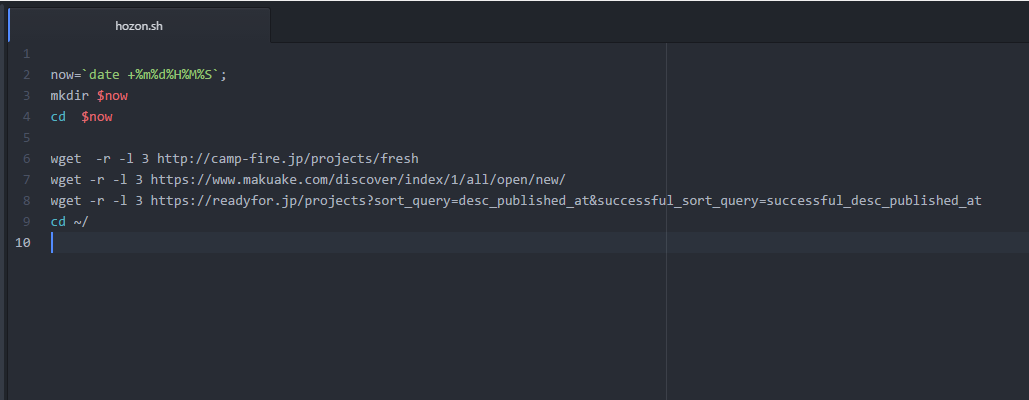
\includegraphics[width=12cm]{hozon1.PNG}
\caption{クローラーの導入1}\label{サンプル図}
\end{figure}
毎日,同時刻にデータを収集する際に,同じフォルダで保存し続けるのを避けるため,Linux コマンドのdata,cd,mkdir を組み合わせてプログラムが動き出した現在時刻をフォルダ名に設定するようにしてある.wget を利用し,各サイトごとに順番にスタート設定したURL から再帰的にファイルを入手するように設定してある.以下に今回使用したコマンドの解説を記す.

\begin{table}[H]
  \begin{center}
    \caption{[date]日付,時刻を表示,設定する}
    \begin{tabular}{|l|c|} \hline
      文字 & 解説  \\ \hline
\%H & 時 (00~23) \\
\%I & 時 (01~12) \\
\%k & 時 ( 0~23) \\
\%l & 時 ( 1~12) \\
\%M & 分 (00~59) \\
\%p & AM あるいは PM のロケール(国や地域に合わせた文字列) \\
\%r & 12時間形式の時刻 (HH:mm:ss [AP]M) \\
\%s & 1970-01-01 00:00:00 UTC からの秒数 \\
\%S & 秒 (00~61) \\
\%T & 24時間形式の時刻 (HH:mm:ss) \\
\%a & ロケールによる省略形の曜日の名前 (Sun~Sat) \\
\%A & ロケールによる完全に表記した曜日の名前(Sunday~Saturday) \\
\%b & ロケールによる省略形の月の名前 (Jan~Dec) \\
\%B & ロケールによる完全に表記した月の名前(January~December) \\
\%c & ロケールによる日付と時刻 (Sat Nov 04 12:02:33 EST 1989) \\
\%d & 日(月内通算日数) (01~31) \\
\%D & 日付 (MM/DD/YY) \\
\%j & 年内通算日数 (001~366) \\
\%m & 月 (01~12) \\
\%w & 週のうちの曜日(0~6)で0が日曜日に対応 \\
\%x & ロケールによる日付の表現 (MM/DD/YY) \\
\%y & 西暦の下2けた (00~99) \\
\%Y & 年 (1970~) \\ \hline
 \end{tabular}
  \end{center}
\end{table}


\begin{table}[H]
  \begin{center}
    \caption{[cd] ディレクトリを移動する}
    \begin{tabular}{|l|c|} \hline
      文字 & 解説  \\ \hline
   / & ルート・ディレクトリ \\
    . & 現在のディレクトリ \\
   … & 親ディレクトリ \\
  \~/ & ホーム・ディレクトリ \\ \hline
    \end{tabular}
  \end{center}
\end{table}

\begin{table}[H]
  \begin{center}
    \caption{[mkdir] ディレクトリを作成する}
    \begin{tabular}{|l|c|} \hline
      文字 & 解説  \\ \hline
   -m & ディレクトリのモードを設定する \\
    -p & 指定したディレクトリをサブディレクトリごと作成する. \\
   -v & ディレクトリを作成する毎にメッセージを出力する \\
   --help & mkdirコマンドの使用法を表示する \\
--version	& バージョン情報を標準出力に表示する \\
directory & 作成するディレクトリ名を指定する \\ \hline
    \end{tabular}
  \end{center}
\end{table}

\newpage

\begin{figure}[H]
\centering
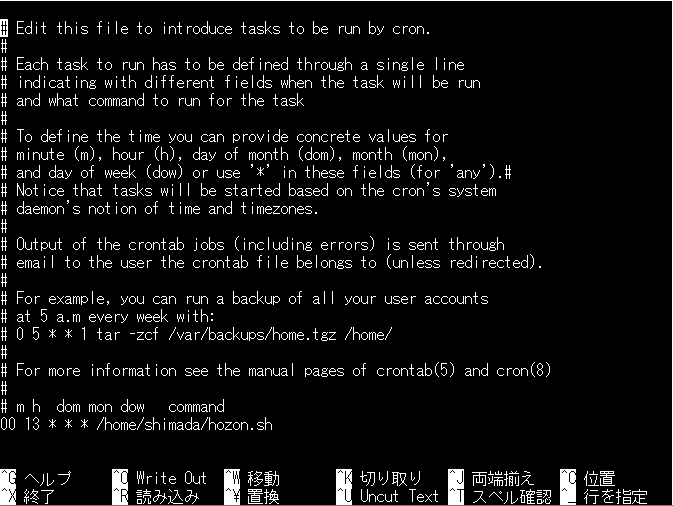
\includegraphics[width=12cm]{hozon2.PNG}
\caption{クローラーの導入2}\label{サンプル図}
\end{figure}

ホーム上にあるシェルを毎日,同じ時間に自動で動かすために,端末からcrontab を利用して時間が来たらシェルを呼び出し,プログラムをスタートするように設定する.
端末を起動し,crontab -u ユーザー名 -e  と入力をし実行する.
実行すると上記の画面が表示される.

エディターでプログラムを行う時刻とプログラムを指定する.文法は以下のとおりである.

分 時 日 月 曜日 コマンド

\begin{table}[H]
  \begin{center}
    \caption{記述方法}
    \begin{tabular}{|l|c|} \hline
      文法 & 解説  \\ \hline
分 & 分を「0~59」で指定する。ワイルドカード(*)を記述すると毎分となる。 \\
時 & 時間を「0~23」で指定する。ワイルドカード(*)を記述すると毎時となる。 \\
日 & 日を「1~31」で指定する。ワイルドカード(*)を記述すると毎日となる。 \\
月 & 月を「1~12」もしくは「jan~dec」で指定する。ワイルドカード(*)を記述すると毎月となる。 \\
曜日 & 曜日を「0~7」(0,7は日曜日)もしくは「sun~sat」で指定する。ワイルドカード(*)を記述すると毎日となる。 \\
コマンド & 実行したいコマンドやシェルを記述します。 \\ \hline
    \end{tabular}
  \end{center}
\end{table}

今回のクローラーの稼働設定を例としてあげると,

00 13 * * * /home/shimada/hozon.sh   

毎日13:00に/home/shimadaにあるhozon.shを実行するという命令になる.

\newpage

\begin{figure}[H]
\centering
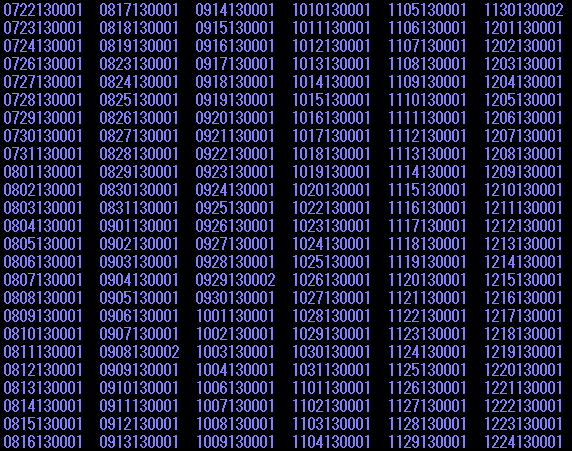
\includegraphics[width=12cm]{hozon3.PNG}
\caption{データが格納されているディレクトリ1}\label{サンプル図}
\end{figure}

実際にデータを集めると上記のようにディレクトリが自動生成される.ディレクトリ名の0722130001は,7月22日13時00分01秒といったようにプログラムを実行した月日時分秒となっている.


\newpage

以下にデータが格納されているディレクトリの構造を記す.

\begin{figure}[H]
\centering
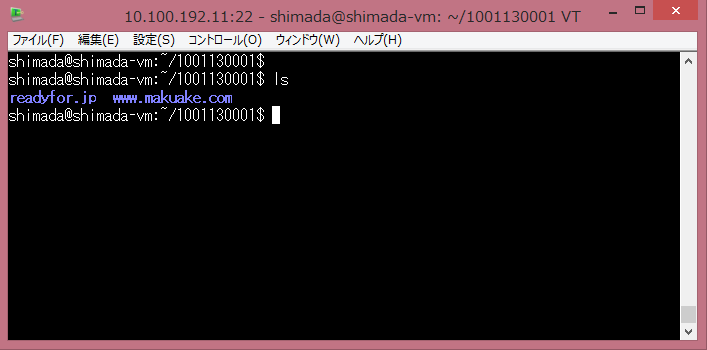
\includegraphics[width=12cm]{hozon4.PNG}
\caption{データが格納されているディレクトリ2}\label{サンプル図}
\end{figure}

\begin{figure}[H]
\centering
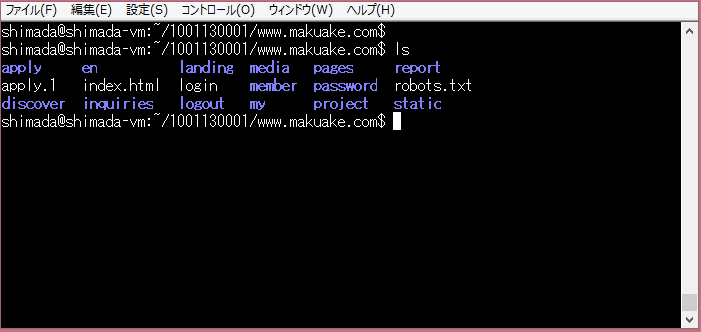
\includegraphics[width=12cm]{hozon5.PNG}
\caption{project内のディレクトリ1}\label{サンプル図}
\end{figure}
\newpage


\begin{figure}[H]
\centering
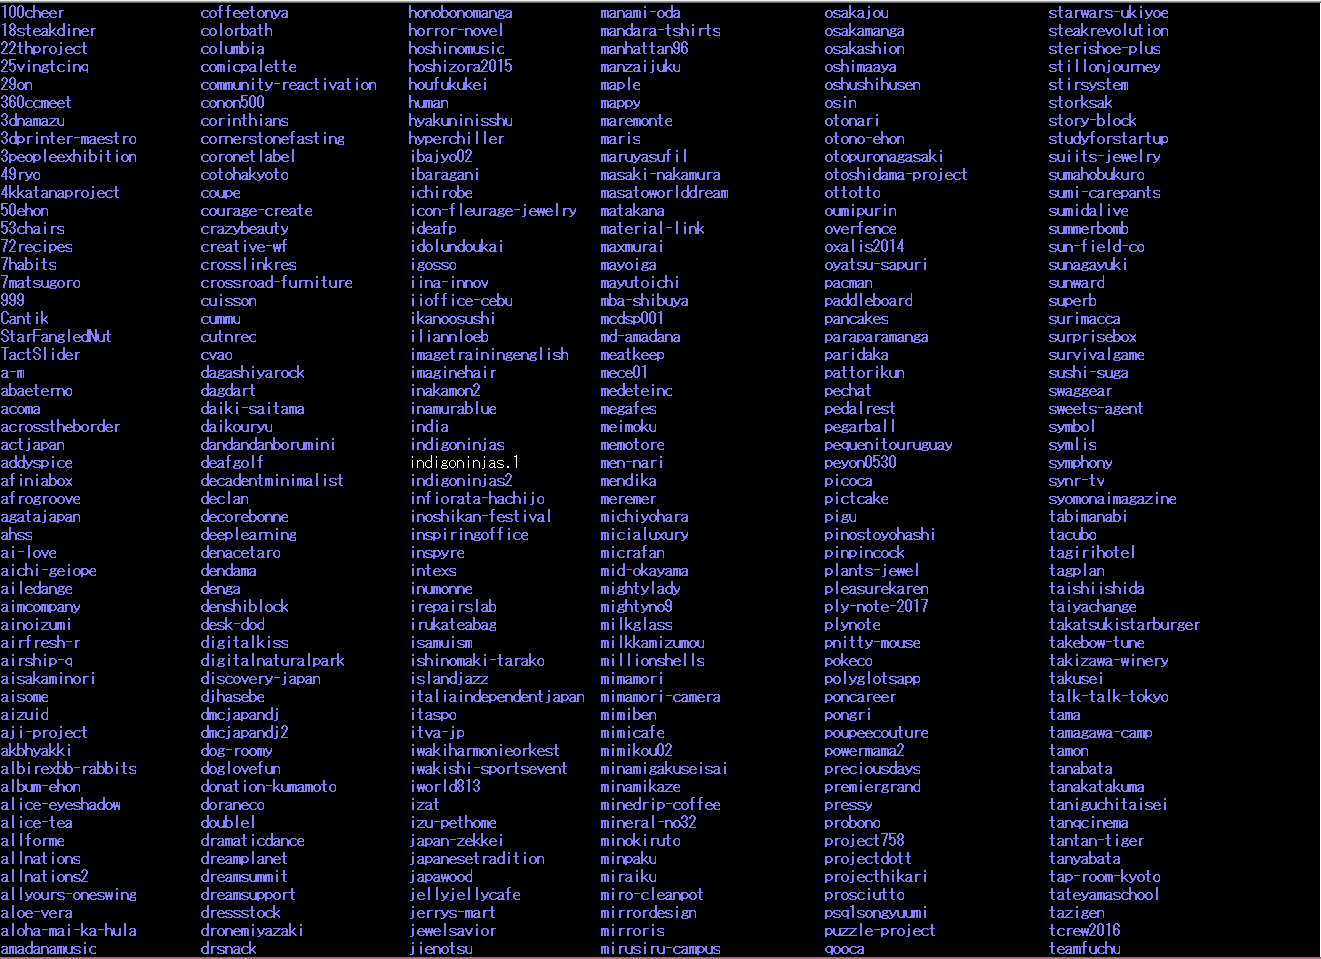
\includegraphics[width=12cm]{hozon6.PNG}
\caption{project内のディレクトリ2}\label{サンプル図}
\end{figure}
\newpage

\begin{figure}[H]
\centering
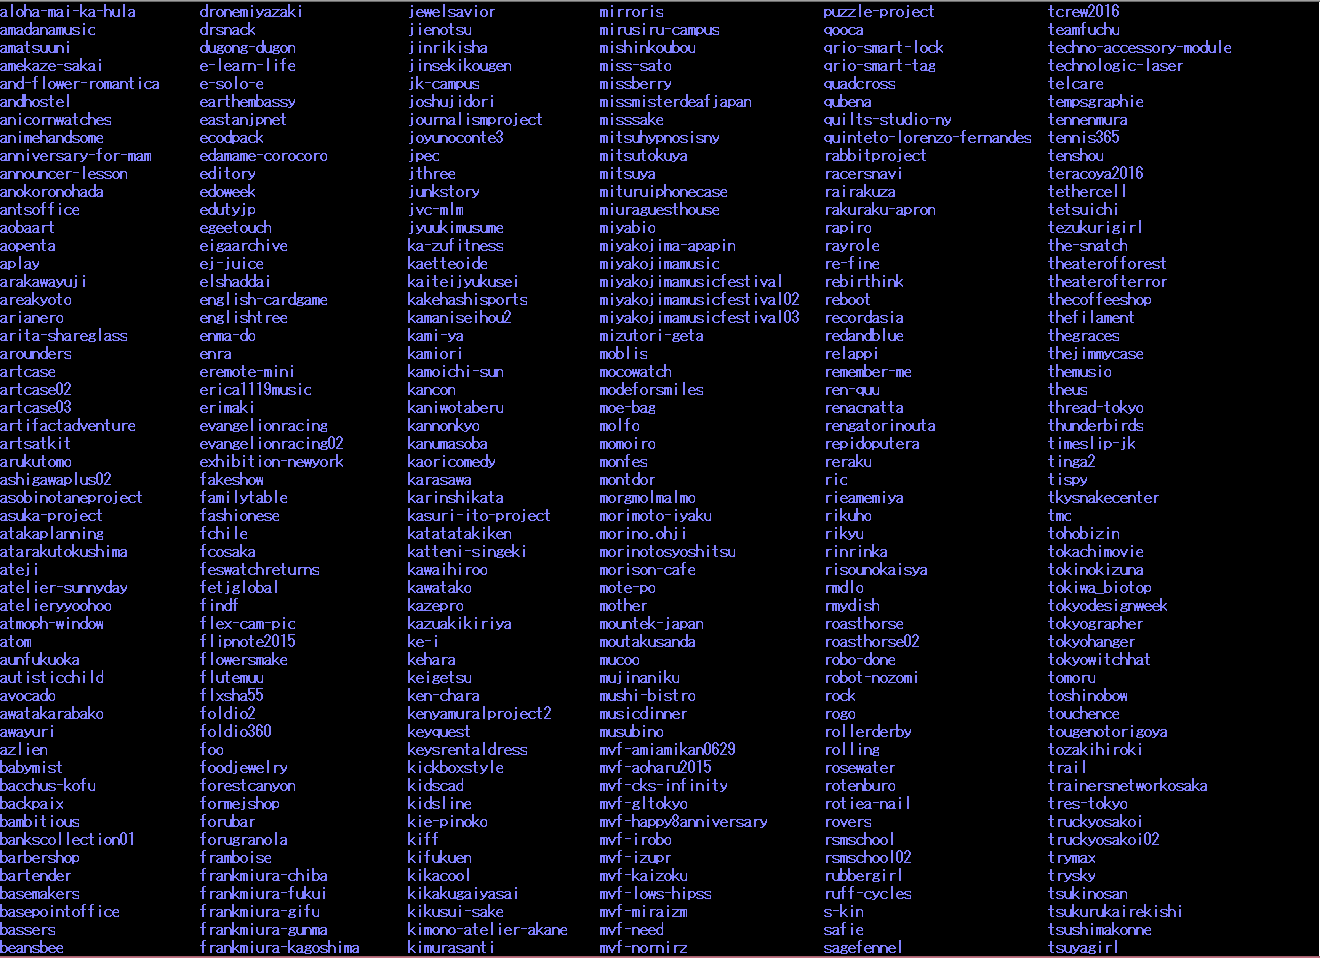
\includegraphics[width=12cm]{hozon7.PNG}
\caption{project内のディレクトリ3}\label{サンプル図}
\end{figure}
\newpage

\begin{figure}[H]
\centering
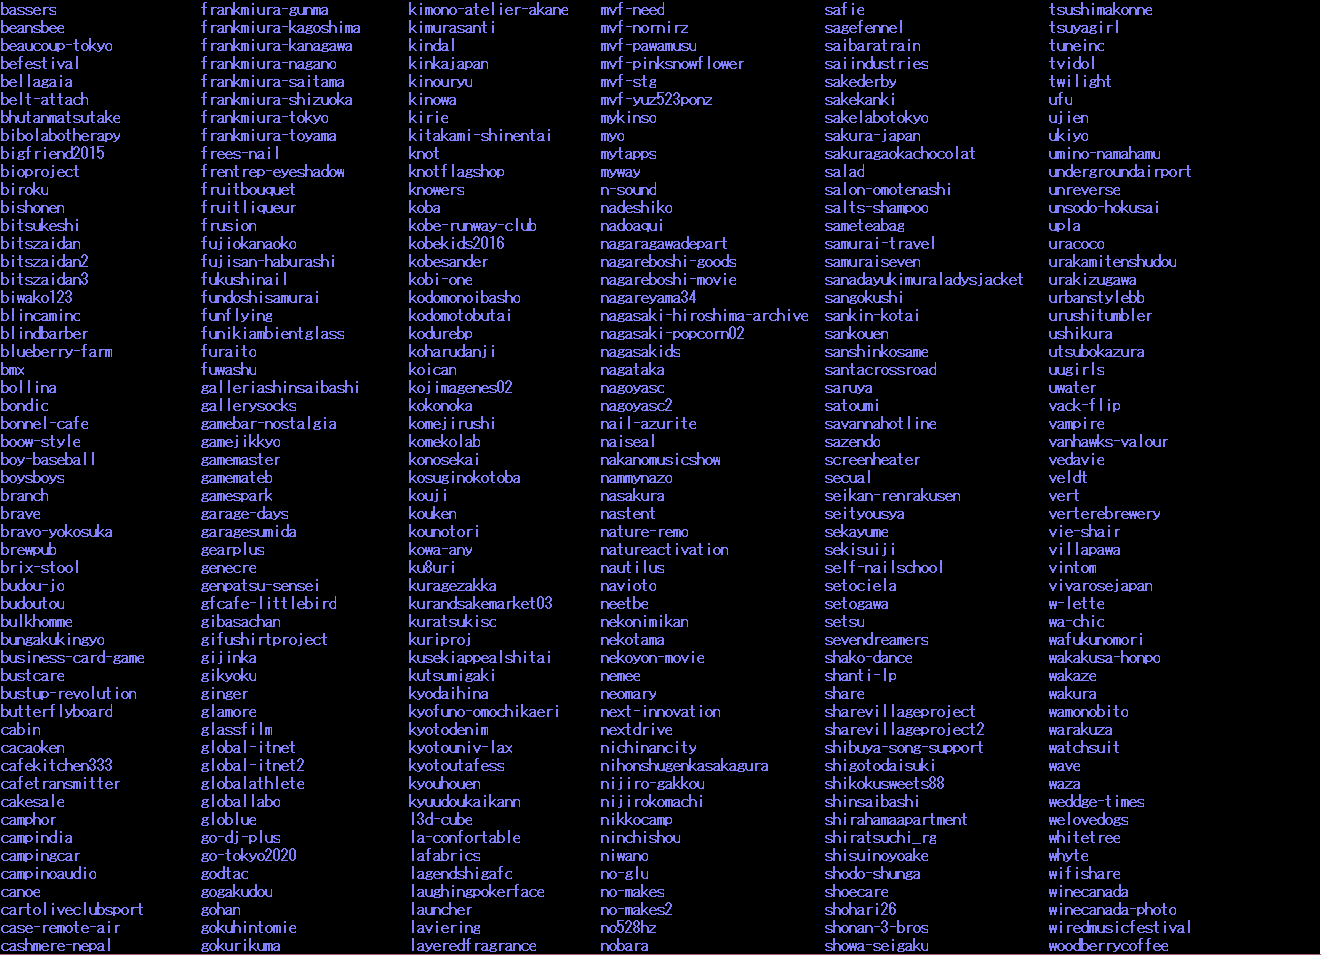
\includegraphics[width=12cm]{hozon8.PNG}
\caption{project内のディレクトリ4}\label{サンプル図}
\end{figure}
\newpage

\begin{figure}[H]
\centering
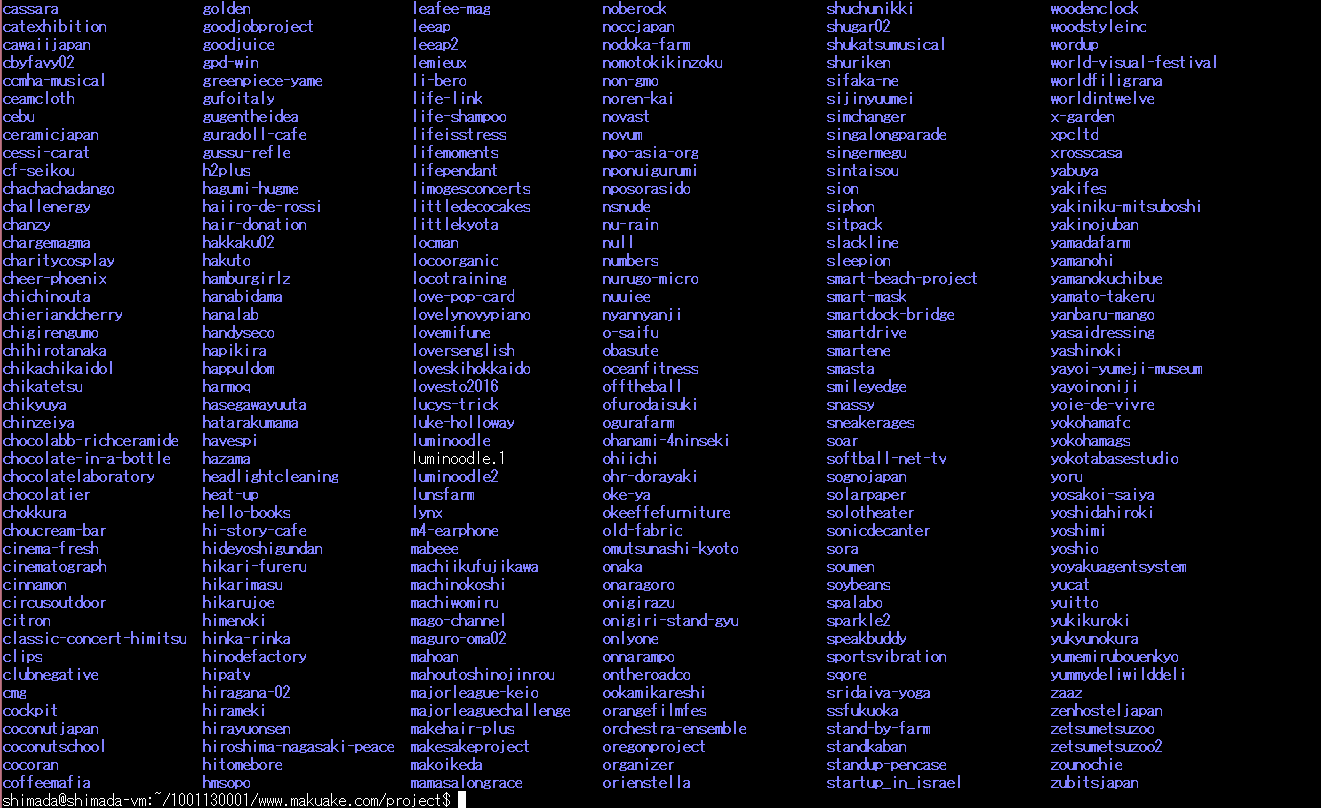
\includegraphics[width=12cm]{hozon9.PNG}
\caption{project内のディレクトリ5}\label{サンプル図}
\end{figure}

これらのディレクトリ名を https://www.makuake.com/project/ のあとに足してweb上で検索することでインターネットに掲載されている状態のプロジェクトを見ることができる.
各ディレクトリ内にあるindex.htmlがその日取得したプロジェクトのデータである.
\newpage
%------------------------------------------------------------------------------------------------------------------------------------------

\section{調査方法}
クローラーを使用し,取得できたデータを処理する.今回取得したデータは2016年7月18日から2017年1月6日までに取得したデータである.



\subsection{データの整理}
1日ごとのデータを1つのファイルにまとめていく.
まず日付の一覧が記載されたファイルを作成するため,集めたデータのある場所で以下のコマンドを実行する.

\begin{verbatim}
ls > ../date.dat
\end{verbatim}



次にプロジェクト名の一覧を作成する.以下のコマンドで実行する.


\begin{verbatim}
for i in `cat date.dat`;do
ls $i/www.makuake.com/project/ >> pmid.dat
done

sort pmid.dat | uniq > project.dat
\end{verbatim}



次にプロジェクトごとのディレクトリを作成する.以下のコマンドを実行する.

\begin{verbatim}
for i in `cat ../project.dat`;do
mkdir $i
done
\end{verbatim}

\newpage
次にプロジェクトページのhtmlファイルからその日の金額だけを抜き出していく.

\begin{figure}[H]
\centering
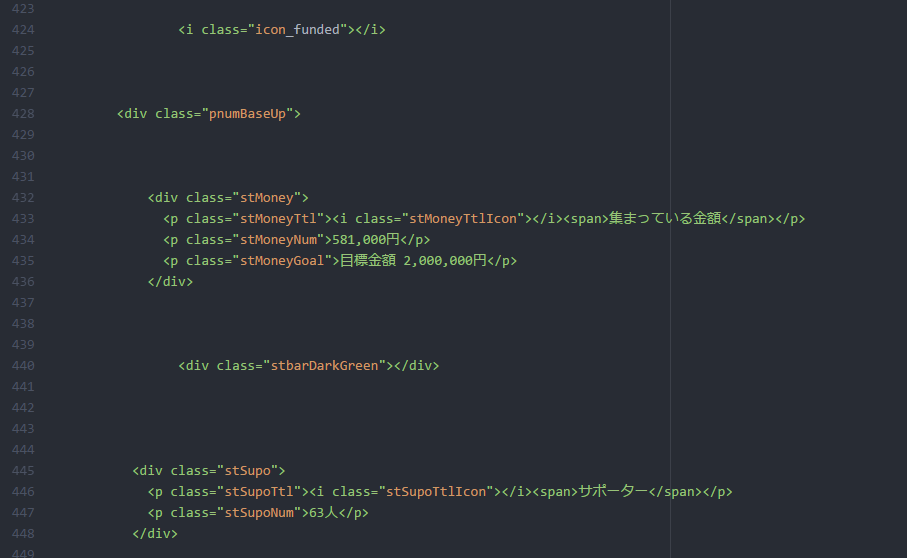
\includegraphics[width=16cm]{P1.PNG}
\caption{取得したプロジェクトページのhtmlファイル}\label{サンプル図}
\end{figure}

上図の581000円の部分である.

作業ディレクトリで以下のコマンドを実行する.

\begin{verbatim}
for d in `cat project.dat`;do
for i in `cat date.dat` ;do
cp ../$i/www.makuake.com/project/$d/index.html $d/$i.html
grep "stMoneyNum" $d/$i.html > $d/$i
gawk -f ed.awk $d/$i > $d/$i.csv
gawk -f ed2.awk $d/$i.csv > $d/$iあ.csv
done
done
\end{verbatim}

\newpage
実行すると各プロジェクトのディレクトリが以下の画像のようになる.

\begin{figure}[H]
\centering
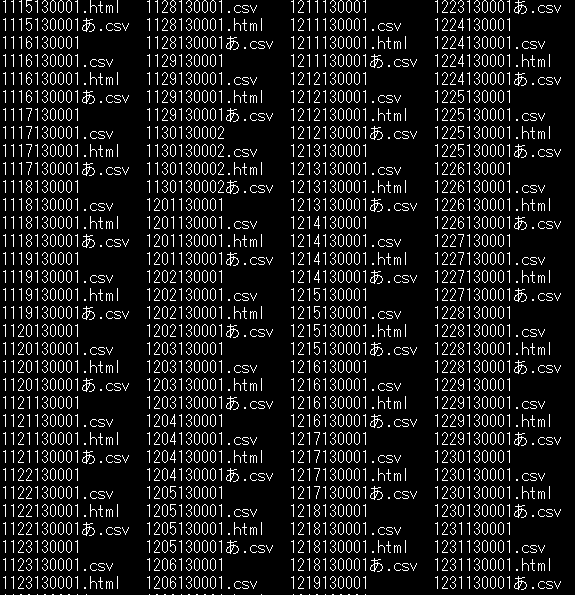
\includegraphics[width=16cm]{seiri1.PNG}
\caption{プロジェクトファイルの中身}\label{サンプル図}
\end{figure}

\newpage
最後に1日ごとの金額のデータを一つのファイルにまとめる.作業ディレクトリで以下のコマンドを実行する.

\begin{verbatim}
for i in `cat project.dat`;do

cat $i/*あ.csv > $i/$i.csv

done

\end{verbatim}


実行すると プロジェクト名.csv というファイルが作成される.
左からプロジェクト名,日付,金額の順でまとめられている.

\newpage
\begin{figure}[H]
\centering
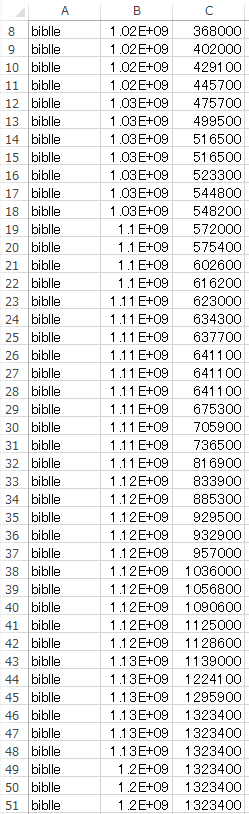
\includegraphics[width=6cm]{P2.PNG}
\caption{プロジェクト名.csv}\label{サンプル図}
\end{figure}

\newpage
\subsection{プロジェクトの選別}
取得したデータから,成功したプロジェクトのみを集める.成功しているかどうかの判断はプロジェクトページの集まっている金額がSuccess!かFundedと表示されているプロジェクトを集める.

\begin{figure}[H]
\centering
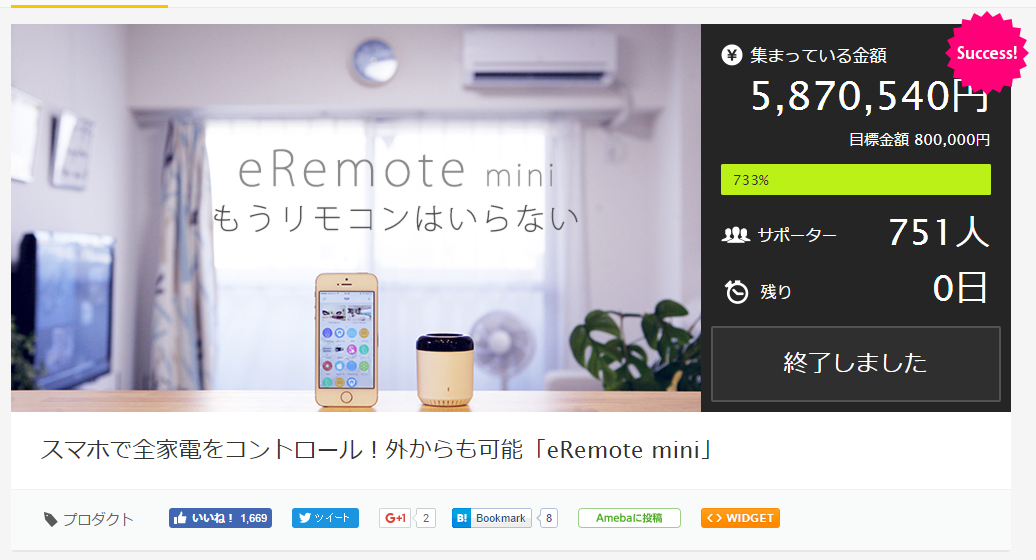
\includegraphics[width=16cm]{senbetu2.PNG}
\caption{Success!と表示されてるプロジェクト}\label{サンプル図}
\end{figure}

\newpage

\begin{figure}[H]
\centering
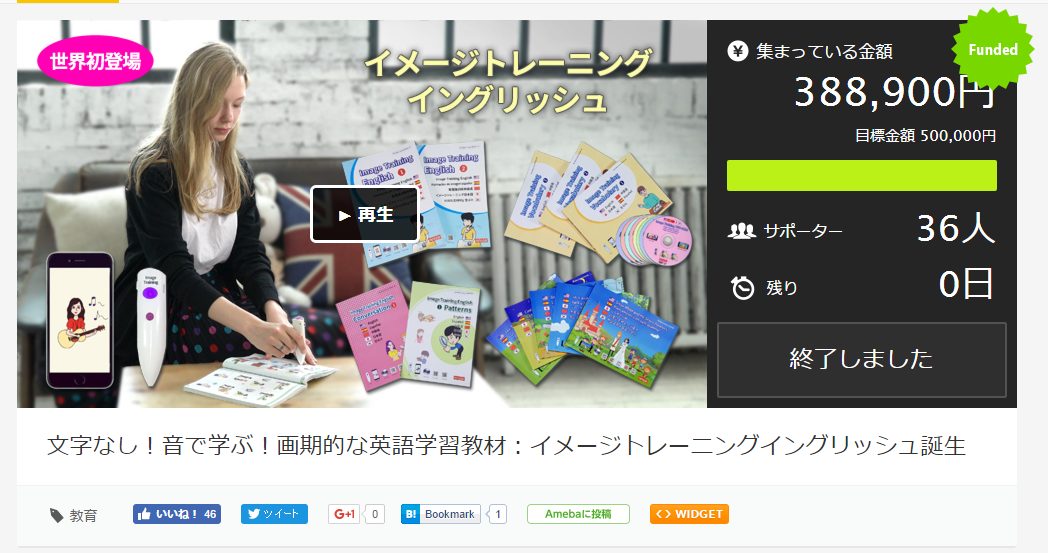
\includegraphics[width=16cm]{senbetu1.PNG}
\caption{Fundedと表示されてるプロジェクト}\label{サンプル図}
\end{figure}



\subsection{ランダムサンプリング}
選別したプロジェクトからランダムサンプリングを行い,データの件数を100件にする.
以下のコマンドを仕訳したファイルのあるディレクトリで実行する.

\begin{verbatim}
shuf -n 100 data.txt
\end{verbatim}

\newpage
\subsection{調達資金の時間変化の可視化}

csvファイルにまとめた調達資金の時間変化を可視化する.
例として,機能性スマートバックパックBACKPAIXのプロジェクトを記載する

\begin{figure}[H]
\centering
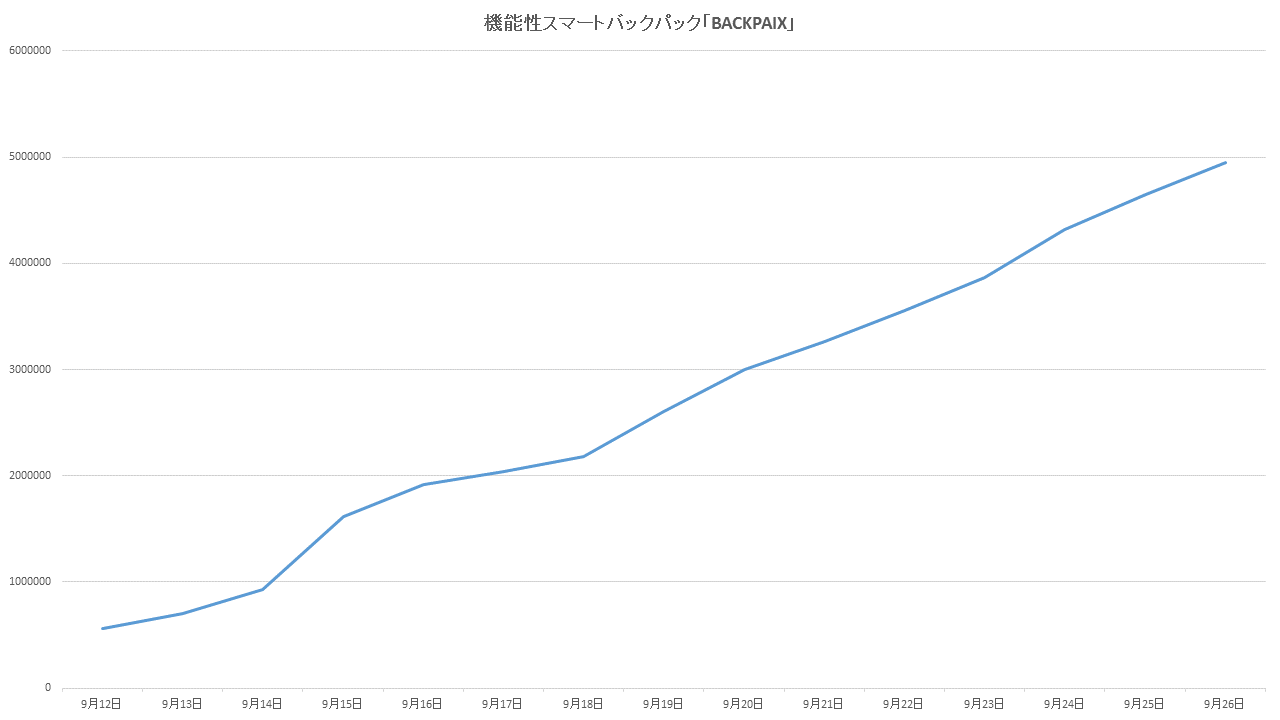
\includegraphics[width=16cm]{chousa1.PNG}
\caption{調達資金の時間変化}\label{サンプル図}
\end{figure}

このグラフから9月14日から9月15日にかけて金額が多く集まっていることがわかる.

\newpage
\subsection{調査項目}

プロジェクト実行者が資金が集まり始める前にしている行動を調査する.調査項目は以下の4項目である.

\begin{enumerate}
 \item サイト内の活動レポートを活用しているか.
 \item 動画を投稿しているか.
 \item Twitterでツイートをしているか.
 \item Facebookで投稿しているか.
\end{enumerate}


\begin{figure}[H]
\centering
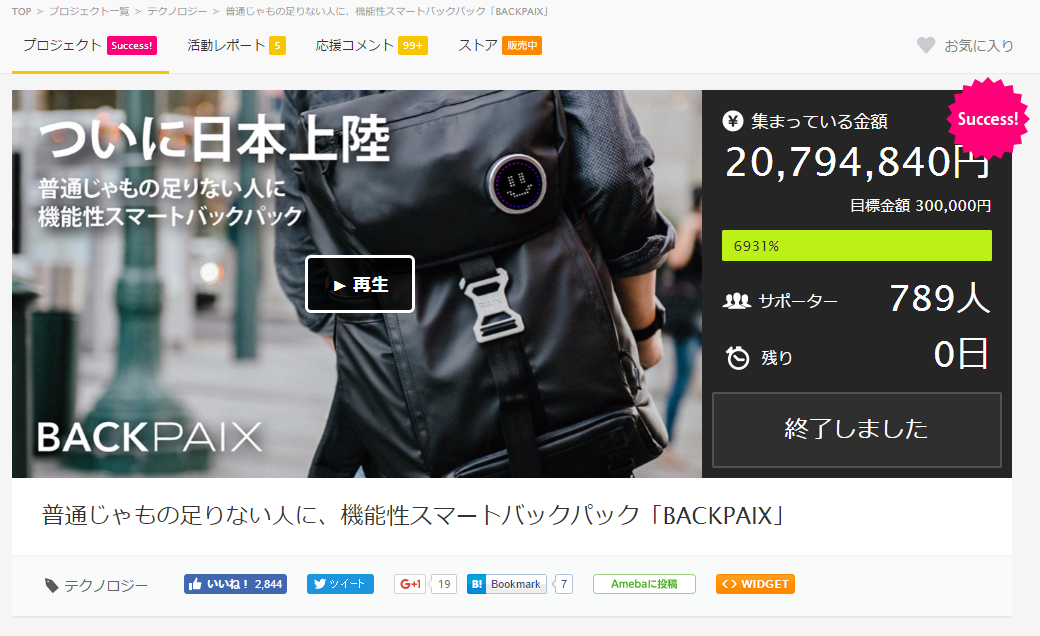
\includegraphics[width=16cm]{chousa2.PNG}
\caption{プロジェクトページ}\label{サンプル図}
\end{figure}

\begin{figure}[H]
\centering
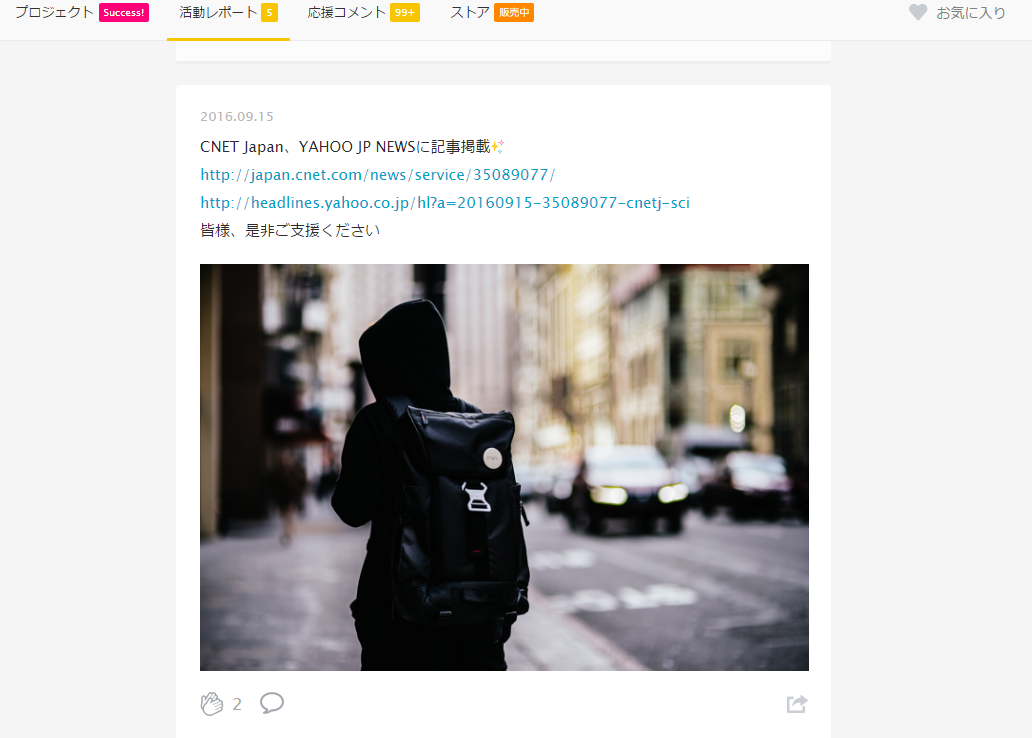
\includegraphics[width=16cm]{chousa3.PNG}
\caption{サイト内の活動レポートページ}\label{サンプル図}
\end{figure}

9月15日に活動レポートを上げていることがわかる.

\begin{figure}[H]
\centering

\includegraphics[width=16cm]{chousa4.PNG}
\caption{プロジェクト実行者のTwitter}\label{サンプル図}
\end{figure}

9月14日にツイートしていることがわかる.

\begin{figure}[H]
\centering

\includegraphics[width=16cm]{chousa5.PNG}
\caption{プロジェクト実行者のFacebook}\label{サンプル図}
\end{figure}

9月14日に投稿していることがわかる.

\begin{figure}[H]
\centering
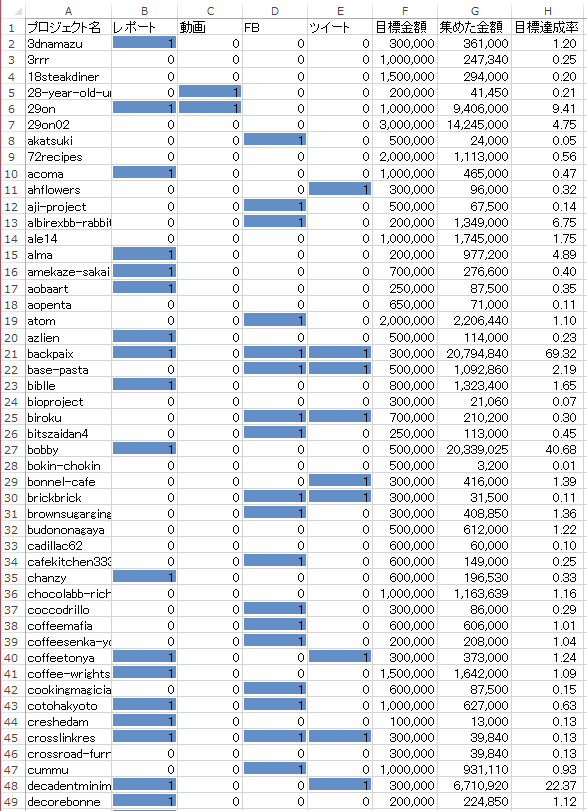
\includegraphics[width=16cm]{chousa6.PNG}
\caption{調査結果のデータ1}\label{サンプル図}
\end{figure}

\begin{figure}[H]
\centering
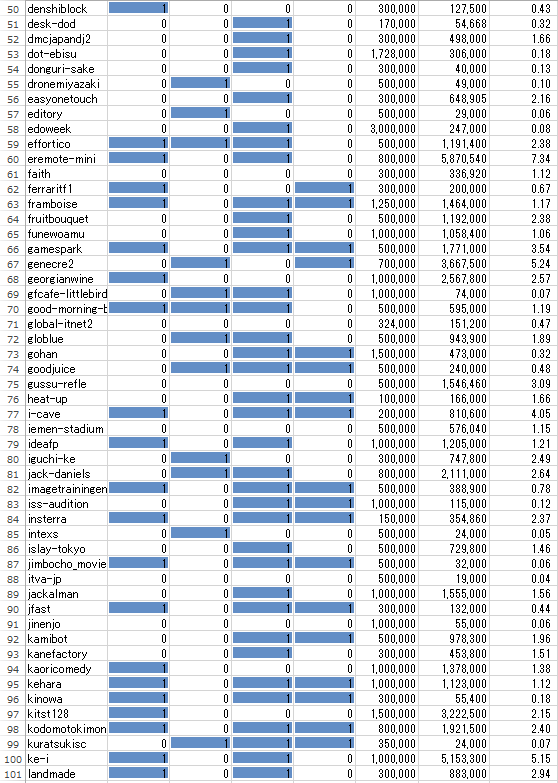
\includegraphics[width=16cm]{chousa7.PNG}
\caption{調査結果のデータ2}\label{サンプル図}
\end{figure}
100件のプロジェクトから調査した4項目と目標金額,集めた金額をExcelにまとめる.集めた金額を目標金額で割り,目標達成率も算出する.


\newpage
\subsection{Rを使用した分析}
Rを使用し,100件のデータから決定木分析を行う.Rで分析を行うにあたって調査結果を分析しやすくしたcsvファイルを作成する.
\begin{figure}[H]
\centering
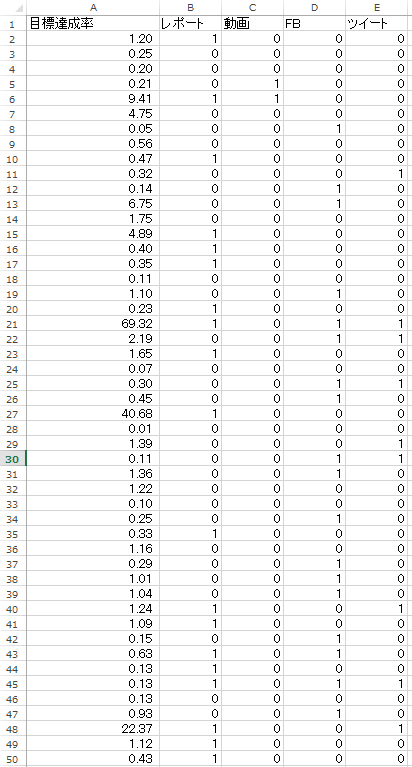
\includegraphics[width=10cm]{keka1.PNG}
\caption{作成したcsvファイル1}\label{サンプル図}
\end{figure}

\begin{figure}[H]
\centering
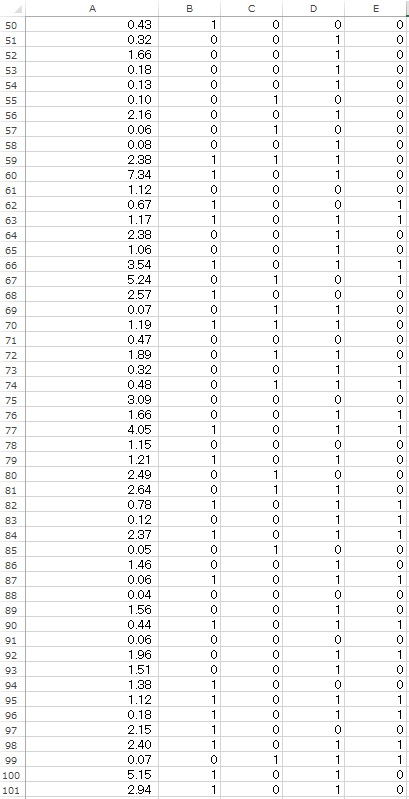
\includegraphics[width=10cm]{keka2.PNG}
\caption{作成したcsvファイル2}\label{サンプル図}
\end{figure}





Cドライブに cit という名前のフォルダを作成し,そこに分析するcsvファイルを置く.


Rを起動し,決定木を作成するのに必要なパッケージをインストールする.
\begin{figure}[H]
\centering
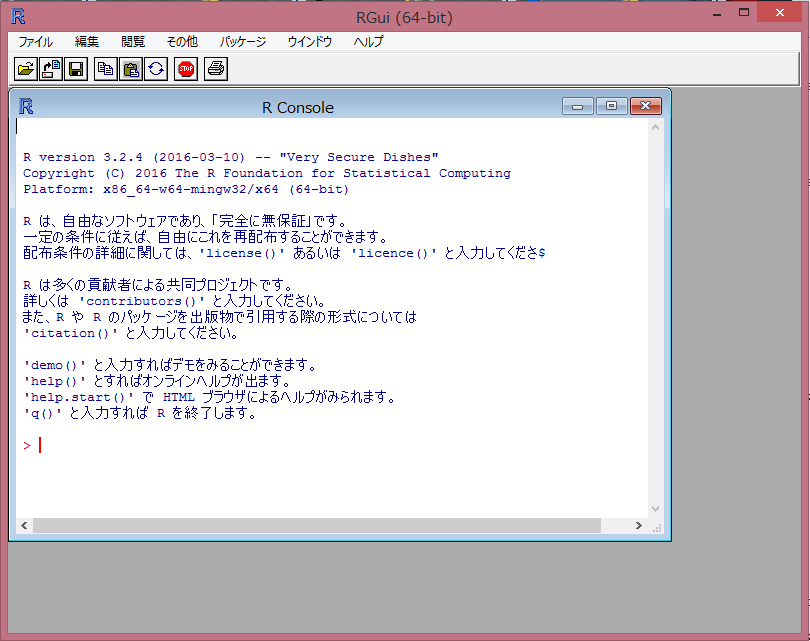
\includegraphics[width=16cm]{R5.PNG}
\caption{起動後のR}\label{サンプル図}
\end{figure}

以下のコマンドを実行する.
\begin{verbatim}
install.packages("rpart")
install.packages("rpart.plot")
\end{verbatim}

\newpage
実行するとサーバーを選択をするのでjapanを選ぶ.

\begin{figure}[H]
\centering
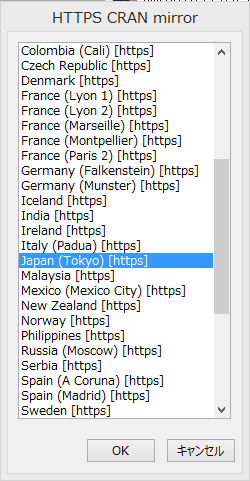
\includegraphics[width=8cm]{R6.PNG}
\caption{サーバーの選択}\label{サンプル図}
\end{figure}

\newpage

\begin{figure}[H]
\centering
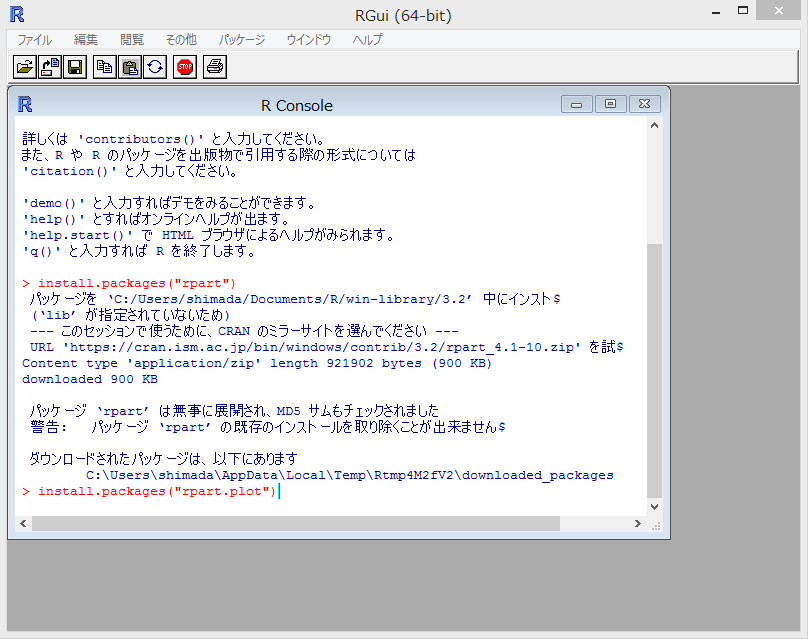
\includegraphics[width=16cm]{R7.PNG}
\caption{インストール完了画面}\label{サンプル図}
\end{figure}
このようになればインストール完了.

\newpage
以下のコマンドを実行し決定木分析を行う.
\begin{verbatim}
library(rpart)
library(rpart.plot)
setwd("C:/cit")
df <- read.csv("keka.csv")
data.rp <- rpart(目標達成率~.,data=df)
\end{verbatim}

\begin{figure}[H]
\centering
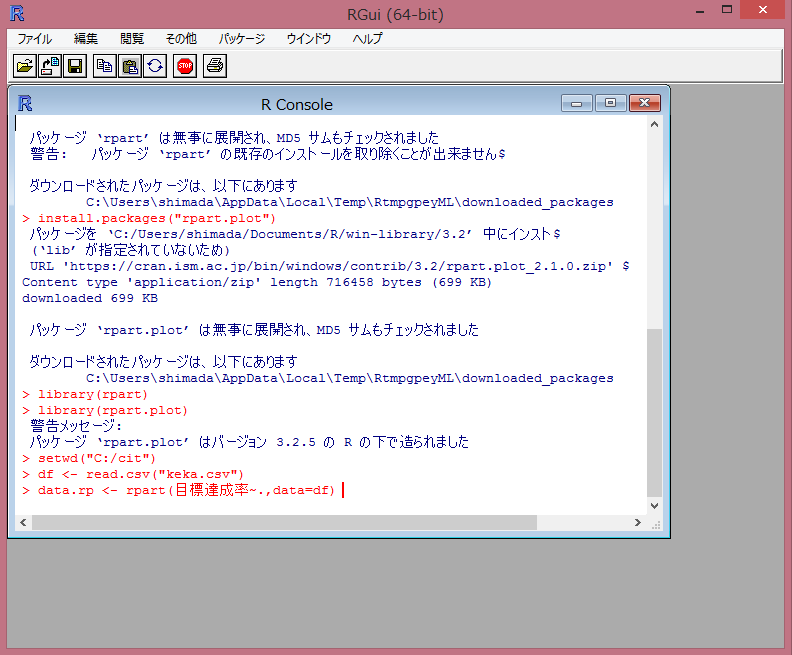
\includegraphics[width=16cm]{R8.PNG}
\caption{決定木分析}\label{サンプル図}
\end{figure}

\newpage
決定木分析の結果をテキストで出力する.
以下のコマンドを実行する.

\begin{verbatim}
print(data.rp)
\end{verbatim}

\begin{figure}[H]
\centering
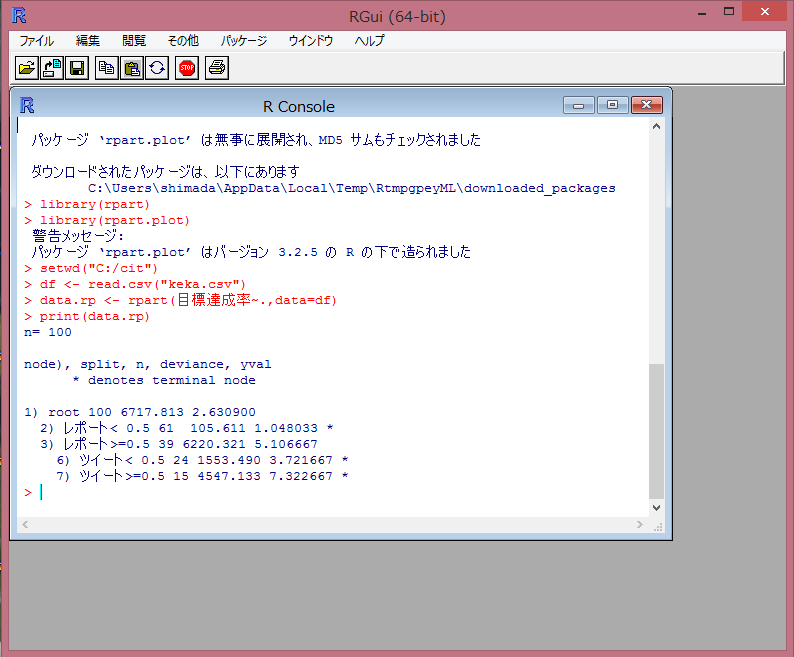
\includegraphics[width=16cm]{R10.PNG}
\caption{テキストで出力}\label{サンプル図}
\end{figure}

最後に決定木を図として出力する.
以下のコマンドを実行する.

\newpage
\begin{verbatim}
rpart.plot(data.rp)
\end{verbatim}

\begin{figure}[H]
\centering
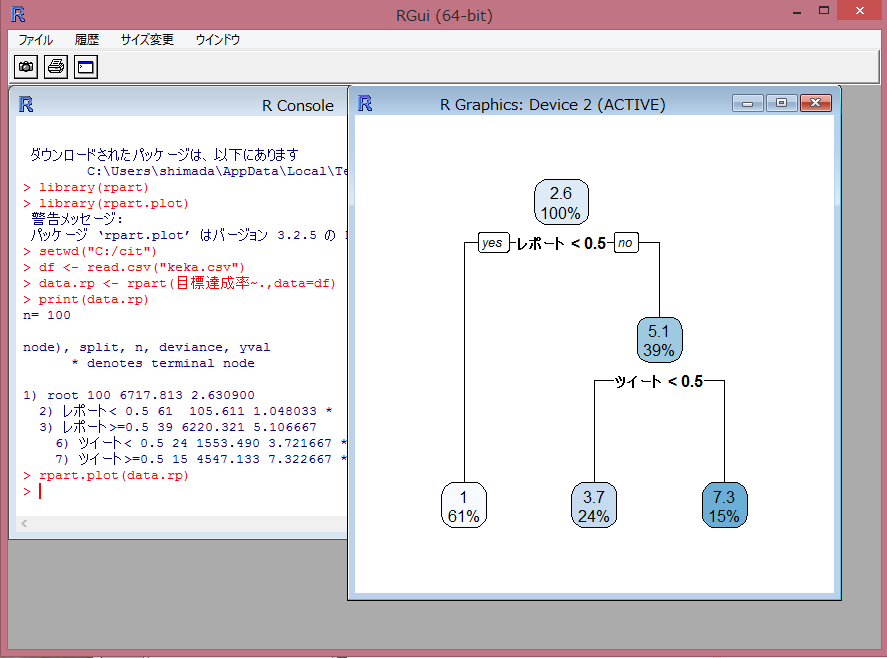
\includegraphics[width=16cm]{R11.PNG}
\caption{図で出力}\label{サンプル図}
\end{figure}
%-------------------------------------------------------------------------------------------------------------------------------------------
\chapter{結果}
目標達成率を目的変数とおいて,レポートとツイートが最も資金調達に関係が深い説明変数となった.

\begin{figure}[H]
\centering
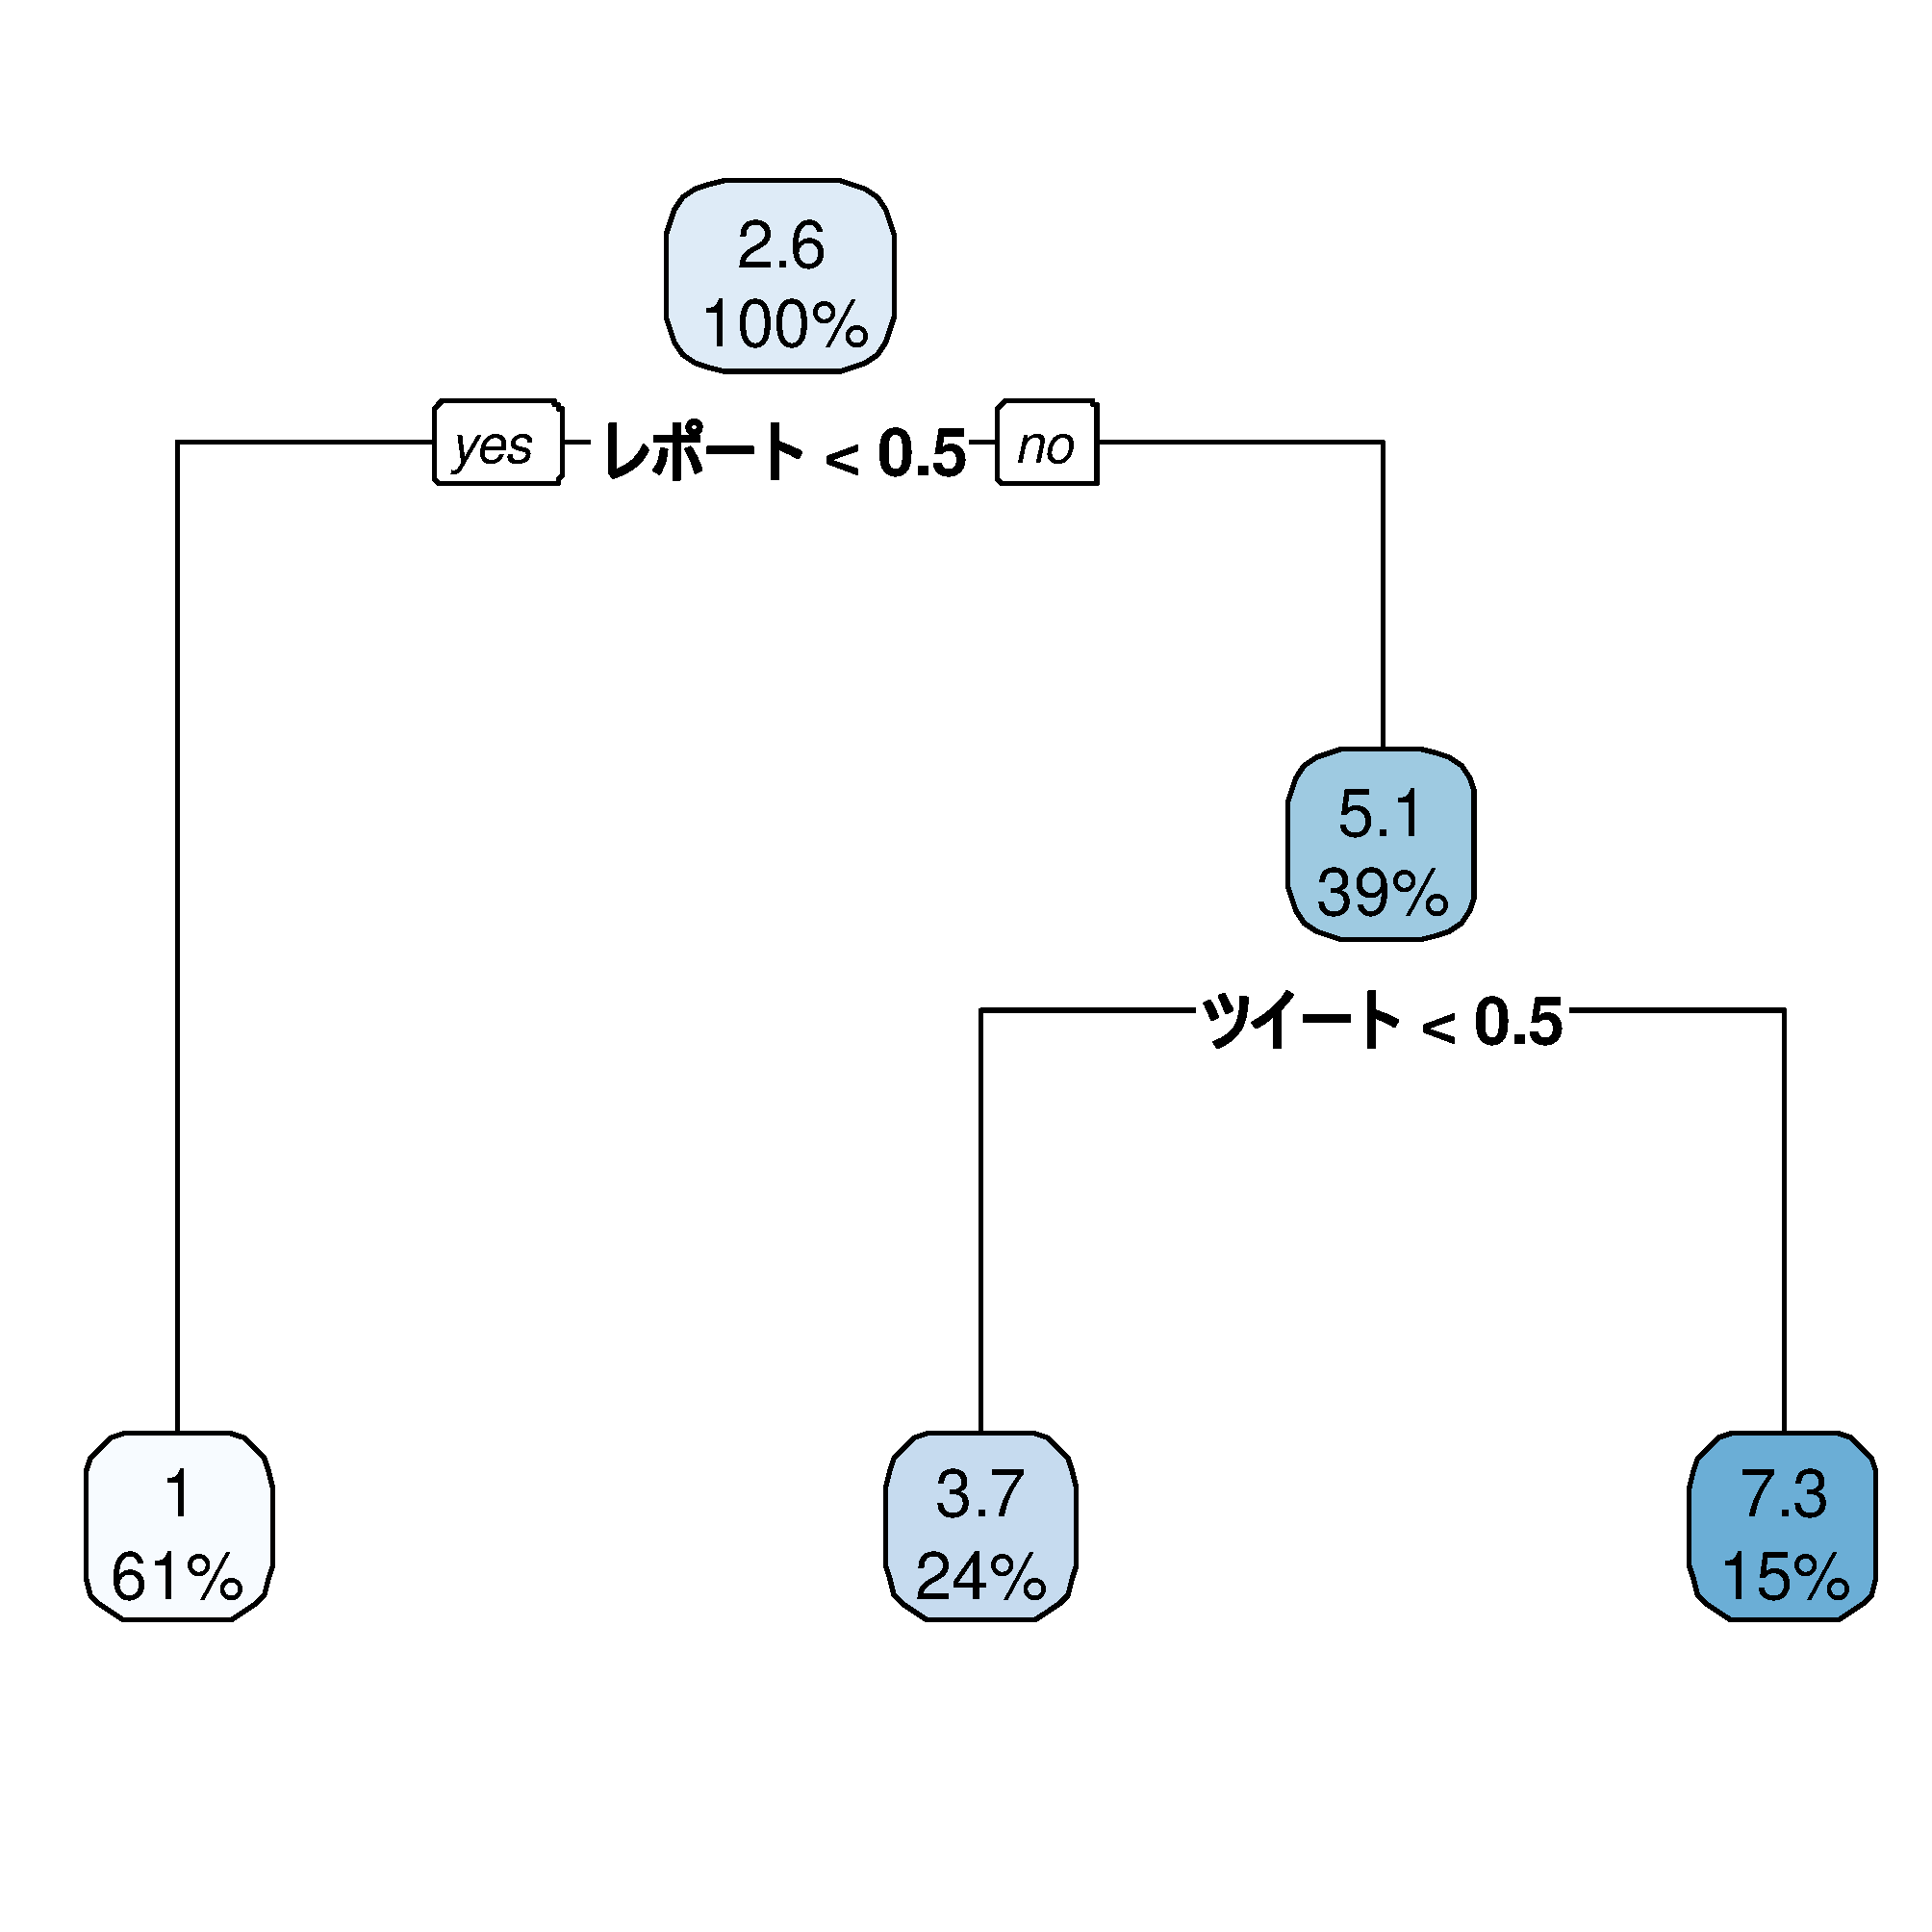
\includegraphics[width=12cm]{ket.PNG}
\caption{決定木分析結果}\label{サンプル図}
\end{figure}
%----------------------------------------------------------------------------------------------------------
\chapter{考察}
レポートとツイートをしてるプロジェクトが資金の調達に最も成功していることがわかる.レポートはプロジェクトのページからすぐに閲覧可能なため,支援者の目につきやすいからだと考えられる.ツイートに関しては,情報の拡散力の高いTwitter によって多数の支援者の目に留まり資金が集まったと考えられる.


\chapter{結論}
本研究で,クラウドファンディングにおいて資金調達する際にプロジェクト実行者がするべき行動はレポートとツイートであるという結果が出た.上記の項目以外に資金調達に関係があると思われる項目を増やしていくことで,さらに精度の高い結果を得られるはずだ.







\bibliographystyle{junsrt}
\bibliography{biblio}%「biblio.bib」というファイルが必要.

\chapter*{謝辞}\addcontentsline{toc}{chapter}{謝辞}
本研究を進めるにあたり,矢吹研究室矢吹太朗准教授には,多くの時間をご指導にさいて頂きました.また,先行研究を行った三浦泰介先輩をはじめ矢吹研究室の皆様には,多くの知識や示唆を頂きました.
協力していただいた皆様に感謝の気持ちと御礼を申し上げます.
\end{document}
